\subsection{约化范数与约化迹的传递性}

命题 7. —— 设 L 是 A 的一个极大交换半单子代数，a 是 L 的一个元素。我们有

\[
\mathrm{Pcrd} _ {\mathrm{A/K}} (a; \mathrm{X}) = \mathrm{Pc} _ {\mathrm{L/K}} (a; \mathrm{X}),\tag{52}
\]

\[
\mathrm{Trd} _ {\mathrm{A/K}} (a) = \mathrm{Tr} _ {\mathrm{L/K}} (a),\tag{53}
\]

\[
\mathrm{Nrd} _ {\mathrm{A/K}} (a) = \mathrm{N} _ {\mathrm{L/K}} (a).\tag{54}
\]

由 VIII, 第 262 页，命题 3，L-模 A 与 \(L^{n}\) 同构；因此我们有关系式

\[
\mathrm{Pc} _ {\mathrm{A/K}} (a; \mathrm{X}) = \mathrm{Pc} _ {\mathrm{L/K}} (a; \mathrm{X}) ^ {n}.
\]

由于多项式 \(\mathrm{Pc}_{\mathrm{L}/\mathrm{K}}(a;\mathrm{X})\) 是首一的，它于是等于约化特征多项式 \(\mathrm{Pcrd}_{\mathrm{A}/\mathrm{K}}(a;\mathrm{X})\)（VIII, 第 339 页，引理 2）；这就给出公式 (52)。比较 (52) 两边 \(X^{n-1}\) 的系数（相应地，常数项），我们便得到公式 (53)（相应地，(54)）。

推论. —— 设 D 是 K 上的一个有限次数的体，其中心为 K。设 a 是 K 的一个元素，L 是 D 的一个包含 a 的极大交换子域。我们有

\[
\begin{array}{c} \mathrm {Pcrd_ {D / K}} (a; \mathrm{X}) = \mathrm {Pc_ {L / K}} (a; \mathrm{X}), \\ \mathrm{Tr} _ {\mathrm{D/K}} (a) = \mathrm{Tr} _ {\mathrm{L/K}} (a), \\ \mathrm{Nrd} _ {\mathrm{D/K}} (a) = \mathrm{N} _ {\mathrm{L/K}} (a). \end{array}\tag{55}
\]

事实上，由 VIII, 第 265 页，推论 2，D 的极大交换子域 L 是 D 的一个极大交换半单子代数。

命题 8. —— 设 B 是 A 的一个单子代数。用 L 表示 B 的中心，用 B' 表示 B 在 A 中的交换子。那么 B' 是体 L 上的一个中心单代数；我们用 r 表示它的约化次数。对 B 的每个元素 b，我们有关系式

\[
\mathrm{Pcrd} _ {\mathrm{A/K}} (b; \mathrm{X}) = \mathrm{N} _ {\mathrm{L[X]/K[X]}} (\mathrm{Pcrd} _ {\mathrm{B/L}} (b; \mathrm{X})) ^ {r},\tag{56}
\]

\[
\mathrm{Trd} _ {\mathrm{A/K}} (b) = r \mathrm{Tr} _ {\mathrm{L/K}} (\mathrm{Trd} _ {\mathrm{B/K}} (b)),\tag{57}
\]

\[
\mathrm{Nrd} _ {\mathrm{A/K}} (b) = \mathrm{N} _ {\mathrm{L/K}} (\mathrm{Nrd} _ {\mathrm{B/L}} (b)) ^ {r}.\tag{58}
\]

引理 6. —— 设 \(\mathbf{K}'\) 是一个有限次数为 \(d\) 的交换 \(\mathbf{K}\)-代数，并设

\[
\mathrm{P} (\mathrm{X}) = \mathrm{X} ^ {s} + a _ {1} \mathrm{X} ^ {s - 1} + \dots + a _ {s}
\]

是一个系数属于 \(K'\) 的首一多项式。那么多项式 \(Q = N_{K'[X]/K[X]}(P)\) 在 \(K[X]\) 中是首一的，次数为 sd，\(X^{sd-1}\) 在 \(Q(X)\) 中的系数等于 \(\mathrm{Tr}_{\mathrm{K}'/\mathrm{K}}(a_1)\)，且 Q 的常数项为 \(N_{K'/K}(a_s)\)。

我们把 \(K^{\prime}\)-代数 \(\mathrm{K}^{\prime}[\mathrm{T}]/( \mathrm{P}(\mathrm{T}))\) 记作 \(K^{\prime\prime}\)，并把 T 在 \(K^{\prime\prime}\) 中的典范类记作 t。序列 \((1, t, \ldots, t^{s-1})\) 是 \(K^{\prime\prime}\) 在 \(K^{\prime}\) 上的一组基，而由 t 作乘法在这组基下的矩阵形如

\[
\tau = \left( \begin{array}{c c c c c} 0 & 0 & \dots & 0 & - a _ {s} \\ 1 & 0 & \dots & 0 & - a _ {s - 1} \\ 0 & 1 & \dots & 0 & - a _ {s - 2} \\ . & . & \dots & . & . \\ . & . & \dots & . & . \\ 0 & . & \dots & 1 & - a _ {1} \end{array} \right).\tag{59}
\]

\(XI_{n}-\tau\) 的行列式可对 s 作归纳、按第一行展开来计算。我们得到 \(\det(\mathrm{X}I_{n}-\tau)=\mathrm{P}(\mathrm{X})\)。换言之，我们有 \(\mathrm{P}(\mathrm{X})=\mathrm{P}\mathrm{c}_{\mathrm{K}^{\prime\prime}/\mathrm{K}^{\prime}}(t;\mathrm{X})\)。特别地，\(\mathrm{Tr}_{\mathrm{K}^{\prime\prime}/\mathrm{K}^{\prime}}(t)=-a_{1}\)，且 \(\mathrm{N}_{\mathrm{K}^{\prime\prime}/\mathrm{K}^{\prime}}(t)=(-1)^{s}a_{s}\)。由传递公式（III, §9, No.~4, 第 548 页，推论），我们有

\[
\begin{array}{r} \mathrm{Tr} _ {\mathrm{K} ^ {\prime \prime} / \mathrm{K}} (t) = - \mathrm{Tr} _ {\mathrm{K} ^ {\prime} / \mathrm{K}} (a _ {1}), \quad \mathrm{N} _ {\mathrm{K} ^ {\prime \prime} / \mathrm{K}} (t) = (- 1) ^ {s d} \mathrm{N} _ {\mathrm{K} ^ {\prime} / \mathrm{K}} (a _ {s}), \\ \mathrm{Q} (\mathrm{X}) = \mathrm{Pc} _ {\mathrm{K} ^ {\prime \prime} / \mathrm{K}} (t; \mathrm{X}). \end{array}
\]

另一方面，\([K'' : K] = [K'' : K'][K' : K] = sd\)，因此 \(Q(X)\) 是次数为 sd 的首一多项式。由此便得引理 6。

我们来证明命题 8。由于环 B 是单的，其中心 L 是一个体（VIII, 第 121 页，推论 1）。由 VIII, 第 259 页，定理 5，B 在 A 中的交换子 \(B'\) 是一个以 L 为中心的单环，且我们有等式 \([A:K]=[B:K][B':K]\)。我们用 r 表示 \(B'\) 在 L 上的约化次数，用 s 表示 B 在 L 上的约化次数，用 d 表示 L 在 K 上的次数。我们有

\[
[ \mathrm{A}: \mathrm{K} ] = n ^ {2}, [ \mathrm{B} ^ {\prime}: \mathrm{K} ] = r ^ {2} d, [ \mathrm{B}: \mathrm{K} ] = s ^ {2} d,
\]

因而 \(n^{2}=r^{2}s^{2}d^{2}\)，即 n=rsd。

设 \(b\) 是 B 的一个元素，\(\mathrm{P}(\mathrm{X})\) 是它在 L-代数 B 上的约化特征多项式；它是次数为 \(s\) 的首一多项式。由引理 6，多项式 \(\mathrm{Q} = \mathrm{N}_{\mathrm{L}[\mathrm{X}] / \mathrm{K}[\mathrm{X}]}(\mathrm{P})\) 是次数为 \(sd\) 的首一多项式。因此多项式 \(\mathrm{R} = \mathrm{Q}^r\) 是次数为 \(rsd = n\) 的首一多项式。仍由引理 6，\(\mathrm{X}^{n - 1}\) 在 \(\mathrm{R}(\mathrm{X})\) 中的系数等于 \(-r\operatorname{Tr}_{\mathrm{L} / \mathrm{K}}(\operatorname{Trd}_{\mathrm{B} / \mathrm{L}}(b))\)，而 \(\mathrm{R}(\mathrm{X})\) 的常数项是 \((\mathrm{N}_{\mathrm{L} / \mathrm{K}}((-1)^s\mathrm{Nrd}_{\mathrm{B} / \mathrm{L}}(b)))^r = (-1)^n\mathrm{N}_{\mathrm{L} / \mathrm{K}}(\mathrm{Nrd}_{\mathrm{B} / \mathrm{L}}(b))^r\)。

由于 \([A:K]=r^{2}d[B:K]\)，左 B-模 A 是秩为 \(r^{2}d\) 的自由模（VIII, 第 124 页，命题 5）。因此我们有

\[
\mathrm{Pc} _ {\mathrm{A/K}} (b; \mathrm{X}) = \mathrm{Pc} _ {\mathrm{B/K}} (b; \mathrm{X}) ^ {d r ^ {2}}.\tag{60}
\]

由 III, §9, No.~4, 第 548 页的推论，我们有

\[
\mathrm{Pc} _ {\mathrm{B/K}} (b; \mathrm{X}) = \mathrm{N} _ {\mathrm{L[X] / K[X]}} (\mathrm{Pc} _ {\mathrm{B/L}} (b; \mathrm{X})),\tag{61}
\]

而由于 \(P(X)\) 是 b 在 L-代数 B 上的约化特征多项式，我们有

\[
\mathrm{Pc} _ {\mathrm{B/L}} (b; \mathrm{X}) = \mathrm{P(X)} ^ {s}.\tag{62}
\]

最后，由公式 (60)---(62) 以及 R(X) 的定义，我们有

\[
\mathrm{Pc} _ {\mathrm{A/K}} (b; \mathrm{X}) = \mathrm{N} _ {\mathrm{L[X]/K[X]}} (\mathrm{P(X)}) ^ {d r ^ {2} s} = \mathrm{Q(X)} ^ {d r ^ {2} s} = \mathrm{R(X)} ^ {r s d} = \mathrm{R(X)} ^ {n}\tag{63}
\]

于是 \(\mathrm{R}(\mathrm{X})\) 是 b 在 K-代数 A 上的约化特征多项式。

我们已经证明了公式 (56)。公式 (57) 与 (58) 立即由公式 (56) 和引理 6 得出，因为 \(\mathrm{X}^{n - 1}\) 在 \(\mathrm{Pcrd}_{\mathrm{A / K}}(b;\mathrm{X})\) 中的系数等于 \(-\mathrm{Trd}_{\mathrm{A / K}}(b)\)，而常数项是 \((-1)^n\mathrm{Nrd}_{\mathrm{A / K}}(b)\)。

\subsection{约化范数与行列式}

在本小节中，D 是 K 上的一个有限次数的体，其中心为 K。我们用 \(D_{ab}^{*}\) 表示乘法群 \(D^{*}\) 对其导群（换位子群）的商群，用 \(\pi\) 表示从 \(D^{*}\) 到 \(D_{ab}^{*}\) 的典范同态。映射 \(Nrd_{D/K}\) 诱导一个从 \(D^{*}\) 到 \(K^{*}\) 的群同态；由于 K 是交换的，这个同态的核包含 \(D^{*}\) 的导群。因此，存在唯一的同态 \(\overline{Nrd}\)（从 \(D_{ab}^{*}\) 到 \(K^{*}\) 的），使得 \(\mathrm{Nrd}_{\mathrm{D/K}}(x)=\overline{\mathrm{Nrd}}\circ\pi(x)\) 对每个 \(x\in D^{*}\) 成立。

命题 9. —— 设 V 是体 D 上的一个有限维右向量空间。设 E 是体 K 上的代数 \(\operatorname{End}_{\mathrm{D}}(\mathrm{V})\)；它是中心单的且为有限次数。对 E 的每个可逆元 u，我们有

\[
\mathrm{Nrd} _ {\mathrm{E/K}} (u) = \overline {{\mathrm{Nrd}}} (\det u)\tag{64}
\]

（\(\det u\) 表示 \(u\) 的行列式；其定义参看 VIII, 第 452 页，命题 2）。

我们用 n 表示 V 在 D 上的维数，并利用 V 在 D 上的一组基把 E 与矩阵代数 \(\mathbf{M}_{n}(\mathrm{D})\) 等同起来。代数 E 的乘法群 \(\mathrm{GL}_{n}(\mathrm{D})\) 由对角矩阵与矩阵 \(\mathrm{B}_{ij}(\lambda)\) 生成（II, §10, No.~13, 第 362 页，推论 1）。因此，命题 9 由下面两个特殊情形得出。

\begin{enumerate}
\def\labelenumi{\Alph{enumi})}
\tightlist
\item
  假设 u 是对角矩阵 \(\mathrm{diag}(a_{1},\ldots,a_{n})\)。对每个 \(1\leqslant i\leqslant n\)，设 \(L_{i}\) 是 D 的一个包含 \(a_{i}\) 的极大交换子域；设 L 是 E 的由形如 \(\mathrm{diag}(t_{1},\ldots,t_{n})\)（其中 \(t_{i}\in L_{i}\)，\(1\leqslant i\leqslant n\)）的对角矩阵所组成的子代数。设 d 是 D 在 K 上的约化次数。我们有 \([L_{i}:K]=d\)（对 \(1\leqslant i\leqslant n\)；VIII, 第 265 页，推论 2）。K-代数 L 同构于 \(L_{1}\times\cdots\times L_{n}\)，因而是次数为 nd 的半单代数；而我们又有 \([E:K]=n^{2}[D:K]=n^{2}d^{2}=[L:K]^{2}\)。由此推出 L 是 E 的一个极大交换半单子代数（VIII, 第 262 页，命题 3）。由 VIII, 第 346 页，命题 7，我们有 \(\mathrm{Nrd}_{\mathrm{E}/\mathrm{K}}(u)=\mathrm{N}_{\mathrm{L}/\mathrm{K}}(u)\)。于是，由 III, §9, No.~3, 第 544 页的公式 (18)，我们有
\end{enumerate}

\[
\begin{array}{c} \mathrm{Nrd} _ {\mathrm{E/K}} (u) = \prod_ {i = 1} ^ {n} \mathrm{N} _ {\mathrm{L} _ {i} / \mathrm{K}} (a _ {i}) = \prod_ {i = 1} ^ {n} \mathrm{Nrd} _ {\mathrm{D/K}} (a _ {i}) \\ = \mathrm{Nrd} _ {\mathrm{D/K}} (a _ {1} \dots a _ {n}) = \overline {{\mathrm{Nrd}}} (\pi (a _ {1} \dots a _ {n}))  . \end{array}
\]

此外，由 VIII, 第 453 页，命题 3，我们有 \(\det u = \pi(a_{1} \cdots a_{n})\)，这在此情形给出了公式 (64)。

\begin{enumerate}
\def\labelenumi{\Alph{enumi})}
\setcounter{enumi}{1}
\tightlist
\item
  假设 u 等于 \(\mathrm{B}_{ij}(\lambda)\)，其中 \(\lambda\) 是 D 的一个元素，i, j 是区间 \([1,n]\) 中两个不同的整数。用 d 表示 D 在 K 上的约化次数，用 M 表示由 V 经标量从 D 到 K 的限制而得到的 K 上的向量空间。那么 M 是一个单 E-模，且我们有
\end{enumerate}

\[
\mathrm{Pc} _ {\mathrm{M/K}} (u; \mathrm{X}) = \mathrm{Pcrd} _ {\mathrm{E/K}} (u; \mathrm{X}) ^ {d}\tag{65}
\]

这由 VIII, 第 341 页的公式 (26) 得出。此外，M 是 K 上维数为 \(nd^2\) 的向量空间，且 \(u - 1_{\mathrm{M}}\) 是 M 的一个幂零自同态；因此我们有

\[
\mathrm{Pc} _ {\mathrm{M/K}} (u; \mathrm{X}) = (\mathrm{X} - 1) ^ {n d ^ {2}}.\tag{66}
\]

比较公式 (65) 与 (66)，我们得到

\[
\mathrm{Pcrd} _ {\mathrm{E/K}} (u; \mathrm{X}) = (\mathrm{X} - 1) ^ {n d}\tag{67}
\]

特别地，\(\mathrm{Nrd}_{\mathrm{E}/\mathrm{K}}(u)=1\)。我们又由 VIII, 第 453 页，命题 3 有 det u=1；因此公式 (64) 在此情形成立。

注. —— 若 E 的元素 u 不可逆，则我们有 \(\mathrm{Nrd}_{\mathrm{E}/\mathrm{K}}(u)=0\)（VIII, 第 340 页，命题 3）。

\BourbakiExercises{习题}

\begin{enumerate}
\def\labelenumi{\arabic{enumi})}
\tightlist
\item
  设 B 是交换域 K 上的一个有限次数代数，b 是 B 的一个元素。
\end{enumerate}

\begin{enumerate}
\def\labelenumi{\alph{enumi})}
\item
  若 \(b\) 是幂零的，则对每个在 K 上有限维的 B-模 M，我们有 \(\mathrm{Tr}_{\mathrm{M / K}}(b) = 0\)。由此推出，若 \(b\) 属于 B 的根，则我们有 \(\mathrm{Tr}_{\mathrm{M / K}}(bc) = 0\)（对每个 \(c \in \mathrm{B}\)）。
\item
  证明：若 \(\operatorname{Tr}_{\mathrm{S}/\mathrm{K}}(bc)=0\) 对每个单 B-模 S 与每个 \(c\in B\) 成立，则 b 属于 B 的根（利用稠密性定理）。
\end{enumerate}

\begin{enumerate}
\def\labelenumi{\arabic{enumi})}
\setcounter{enumi}{1}
\tightlist
\item
  设 B 是交换域 K 上一个次数为 n 的有限代数。对 B 的任一元素 b，用 \(\mathrm{Pm}_{\mathrm{B}/\mathrm{K}}(b;\mathrm{X})\) 表示 b 在 K 上的最小多项式（V, §3, No.~1, 第 16 页）。我们有 \(\mathrm{Pm}_{\mathrm{B}/\mathrm{K}}(b;\mathrm{X})=\mathrm{Pm}_{\mathrm{B}^{\circ}/\mathrm{K}}(b;\mathrm{X})\)。
\end{enumerate}

\begin{enumerate}
\def\labelenumi{\alph{enumi})}
\item
  证明 \(\mathrm{Pm}_{\mathrm{B / K}}(b;\mathrm{X})\) 整除 \(\mathrm{Pc}_{\mathrm{B / K}}(b;\mathrm{X})\)，而后者整除 \((\mathrm{Pm}_{\mathrm{B / K}}(b;\mathrm{X}))^n\)。
\item
  对 K 的每个扩张 L，我们有 \(\mathrm{Pm}_{\mathrm{B}_{(\mathrm{L})}/\mathrm{L}}(1 \otimes b; \mathrm{X}) = \mathrm{Pm}_{\mathrm{B}/\mathrm{K}}(b; \mathrm{X})\)。
\item
  设 \((e_i)_{i\in \mathrm{I}}\) 是 B 在 K 上的一组基，\(\mathbf{Y} = (\mathrm{Y}_i)_{i\in \mathrm{I}}\) 是一族变量。代数 B 关于基 \((e_i)\) 的主多项式（记作 \(\mathrm{P}((e_i);\mathrm{X};\mathbf{Y})\)，或简记为 \(\mathrm{P}(\mathrm{X};\mathbf{Y})\)）是 \(\mathrm{K}(\mathbf{Y})\) 上元素 \(\sum_{i\in \mathrm{I}}\mathrm{Y}_i e_i\)（属于 \(\mathrm{B}_{(\mathrm{K}(\mathbf{Y}))}\)）的最小多项式。*证明它属于 \(\mathrm{K}[\mathrm{X};\mathbf{Y}]\)（参看 AC, VII, §3, n° 5, 第 230 页，引理 1 与定理 2）。
\item
  设 \((e_{i}^{\prime})\) 是 B 在 K 上的另一组基，\((\lambda_{ij})\) 是以 K 为元素的矩阵，使得 \(e_{i} = \sum_{j} \lambda_{ij} e_{j}^{\prime}\)（对 \(i \in I\)）；若令 \(Y_{i}^{\prime} = \sum_{j} \lambda_{ji} Y_{j}\)，则 \(\mathrm{P}((e_{i}); \mathrm{X}; \mathbf{Y}) = \mathrm{P}((e_{i}^{\prime}); \mathrm{X}; \mathbf{Y}^{\prime})\)。设 \(b = \sum_{i} \beta_{i} e_{i}\) 是 B 的一个元素；多项式 \(\mathrm{P}((e_{i}); \mathrm{X}; \beta_{1}, \ldots, \beta_{n})\) 与基 \((e_{i})\) 的选取无关；我们把它称为 b 在 K 上的主多项式。它整除 \(\mathrm{Pc}_{\mathrm{B/K}}(b; \mathrm{X})\)，且是 \(\mathrm{Pm}_{\mathrm{B/K}}(b; \mathrm{X}).*\) 的倍式。
\item
  设 \(B'\) 是另一个有限次数的 K-代数；对适当的基，计算代数 \(B \times B'\) 的主多项式。
\end{enumerate}

\begin{enumerate}
\def\labelenumi{\arabic{enumi})}
\setcounter{enumi}{2}
\tightlist
\item
  \begin{enumerate}
  \def\labelenumii{\alph{enumii})}
  \tightlist
  \item
    设 A 是 K 上的一个有限次数中心单代数。证明 A 的元素 \(a\) 的主多项式是 \(\mathrm{Pcrd}_{\mathrm{A} / \mathrm{K}}(a; \mathrm{X})\)。A 的主多项式（关于 A 在 K 上的一组基）就是 VIII, 第 345 页，引理 4 中所考虑的多项式 P（化归到 \(\mathrm{B} = \mathbf{M}_n(\mathrm{K})\) 的情形）。
  \end{enumerate}
\end{enumerate}

\begin{enumerate}
\def\labelenumi{\alph{enumi})}
\setcounter{enumi}{1}
\tightlist
\item
  设 B 是 K 上的一个绝对半单代数，\(\mathcal{S}\) 是单 B-模的类所成之集。证明 B 的元素 b 的主多项式等于多项式 \(\mathrm{Pc}_{\mathrm{S}/\mathrm{K}}(b;\mathrm{X})\)（S 取遍 \(\mathcal{S}\)）的乘积（化归到 K 代数闭的情形）。
\end{enumerate}

¶ 4) 设 D 是一个体，\(\sigma\) 是 D 的一个自同构，A 是环 D{[}X{]} \(_{\sigma}\)（VIII, 第 11 页），\(n\) 是一个 \(\geqslant 2\) 的整数，\(a\) 是 D 的一个非零元素。把 A 的元素 X \(^{n}\) - \(a\) 记作 \(f\)。\(a)\) 理想 A \(f\) 是双边的，当且仅当 \(\sigma(a) = a\) 且 \(\sigma^{n}(x) = axa^{-1}\)（对每个 \(x \in \mathrm{D}\)）。

\begin{enumerate}
\def\labelenumi{\alph{enumi})}
\setcounter{enumi}{1}
\tightlist
\item
  假设包含在 D 的中心中的 n 次单位根所成的群 \(\mu_{n}\) 是 n 阶循环群且被 \(\sigma\) 固定。设 \(g \in A\) 是一个右除 f 的不可约首一多项式（VIII, 第 22 页，习题 27）。证明 g 的次数 d 整除 n，且 f 是 n/d 个次数为 d 的多项式的乘积。（设 h 是使 \(Ah = \bigcap_{\zeta \in \mu_{n}} Ag_{\zeta}\) 成立的首一多项式，其中 \(g_{\zeta}(X) = g(\zeta X)\)。注意我们必然有 \(h(\zeta X) = h(X)\)（对每个 \(\zeta \in \mu_{n}\)），并由此推出 h = f。然后，对 \(1 \leqslant i \leqslant n/d\)，构造一个元素 \(\zeta_{i}\)（属于 \(\mu_{n}\)）与一个次数为 id 的多项式 \(h_{i}\)，使得 \(Ag_{\zeta_{1}} \cap \cdots \cap Ag_{\zeta_{i}} = Ah_{i}\)，从而应用同引文 b)。
\end{enumerate}

此外，若理想 Af 是双边的，则环 A/Af 是半单的，且其单分量都有相同的长度（注意每个单 \((\mathrm{A}/\mathrm{Af})\)-模同构于模 \(A/Ag_{\zeta}\) 之一）。

\begin{enumerate}
\def\labelenumi{\alph{enumi})}
\setcounter{enumi}{2}
\tightlist
\item
  从现在起假设 b) 的假设成立、理想 A f 是双边的，且 n 是一个素数。由 b) 推出我们处于下述情形之一：
\end{enumerate}

\begin{enumerate}
\def\labelenumi{(\roman{enumi})}
\item
  存在一个 \(b \in D\)，使得 \(a = b^{n}\)，且 \(\sigma\) 是与 b 相伴的内自同构。环 C = A/Af 同构于积环 \(D^{n}\)。
\item
  (i) 的条件不满足，但存在一个 \(c \in \mathrm{D}\)，使得 \(a = \sigma^{n-1}(c)\sigma^{n-2}(c)\ldots\sigma(c)c\)。环 C 是长度为 \(n\) 的单环。
\item
  不存在 D 的元素 c 使得 \(a = \sigma^{n-1}(c) \sigma^{n-2}(c) \cdots \sigma(c) c\)。环 C 是一个体。
\end{enumerate}

在 D 交换的情形，重新得出 VIII, 第 330 页，习题 11 的结果。此外，若 n = 2，则 C 是 D 的在 \(\sigma\) 下不变的子域 K 上的一个四元数代数。

\begin{enumerate}
\def\labelenumi{\alph{enumi})}
\setcounter{enumi}{3}
\item
  证明存在 C 的一个自同构 \(\tau\)，其阶为 \(n\)，且其不变元子域等于 D。在上面的情形 (ii) 与 (iii) 中，D 是 C 的一个伽罗瓦子域（VIII, 第 274 页，习题 16）。
\item
  假设 \(\sigma\) 是与 D 的元素 \(d\) 相伴的内自同构。证明我们有 \(a = d^n z\)，其中 \(z\) 属于 C 的中心 Z，且环 C 同构于张量积 \(\mathrm{D} \otimes_{\mathbb{Z}} \mathrm{Z}[\mathrm{X}] / (\mathrm{X}^n - z)\)。
\item
  假设 \(\sigma\) 不是内自同构。证明 C 的中心是由 Z 中在 \(\sigma\) 下不变的元素所组成的子域。
\end{enumerate}

¶ 5) 设 \(K_{0}\) 是有理分式域 \(\mathbf{Q}(\mathrm{X})\)。设 K 是二次扩张 \(\mathrm{K}_{0}(\rho)\)，其中 \(\rho\) 是一个本原三次单位根，D 是 K 的循环扩张 \(\mathrm{K}(\sqrt[3]{\mathrm{X}})\)，\(\sigma\) 是 D 在 K 上的伽罗瓦群的一个生成元。考虑如习题 4 中那样定义的代数 C，取 n = 3 且 a = 2。

\begin{enumerate}
\def\labelenumi{\alph{enumi})}
\item
  证明 C 是一个以 K 为中心的体，且在 K 上的次数为 9。（要看出 D 没有范数为 2 的元素，化为证明不可能有形如 \(2F^{3} = P^{3} + XQ^{3} + X^{2}R^{3} + 3XPQR\) 的关系，其中 F, P, Q, R 是 \(\mathbf{Q}(\rho)[\mathrm{X}]\) 中两两互素的多项式。为此，考察这些多项式的最低次项。）
\item
  证明不存在 C 的自同构延拓 K 的异于恒同映射的唯一的 \(K_{0}\)-自同构（化归到这样的自同构保持 D 的情形）。由此推出 \(K_{0}\) 不是 C 的伽罗瓦子域（VIII, 第 274 页，习题 16），且不存在 C 的阶为 2 的 \(K_{0}\)-自同构。
\item
  设 \(\xi\) 是 D 的一个使 \(\xi^3 = \mathrm{X}\) 的元素，\(\eta\) 是 C 的一个使 \(\eta^3 = 2\) 且 \(\eta \xi = \rho \xi \eta\) 的元素；令 \(\zeta = \xi + \eta + \eta^2\)。证明 \(\mathrm{K}(\zeta)\) 是 D 的一个极大交换子域且在 K 上不是伽罗瓦的，而极大交换子域 \(\mathrm{K}(\xi)\) 与 \(\mathrm{K}(\eta)\) 在 K 上是伽罗瓦的（计算 \(\zeta^3\)）。
\end{enumerate}

\begin{enumerate}
\def\labelenumi{\arabic{enumi})}
\setcounter{enumi}{5}
\tightlist
\item
  设 D 是一个以 K 为中心、在 K 上的次数为 \(m^{2}\) 的体。设 x 是 D 的一个在 K 上次数为 n（\textgreater{} 1）的元素，\(f(\mathrm{X})\) 是它在 K 上的最小多项式。
\end{enumerate}

\begin{enumerate}
\def\labelenumi{\alph{enumi})}
\item
  证明 D{[}X{]}（VIII, 第 11 页）中一个次数 \textless{} n 的首一多项式不可能被所有多项式 \(X - txt^{-1}\)（\(t \in D^{*}\)）右整除（注意理想 \(\cap(\mathrm{D}[\mathrm{X}](\mathrm{X}-txt^{-1}))\) 的首一生成元的系数属于 K）。
\item
  设 \(u(\mathrm{X}), v(\mathrm{X}), w(\mathrm{X})\) 是 D{[}X{]} 中三个首一多项式，满足 \(u(\mathrm{X}) = v(\mathrm{X})w(\mathrm{X})\)，且 \(\mathrm{X} - x\) 是 \(u(\mathrm{X})\) 的右因子而不是 \(w(\mathrm{X})\) 的右因子。写 \(w(\mathrm{X}) = q(\mathrm{X})(\mathrm{X} - x) + t\)，其中 \(t \in \mathrm{D}^*\)。证明 \(\mathrm{X} - txt^{-1}\) 是 \(v(\mathrm{X})\) 的右因子。
\item
  由 a) 与 b) 推出，存在 D 的 n 个元素 \(t_{1},\ldots,t_{n}\)，使得我们有
\end{enumerate}

\[
f (\mathrm{X}) = \left(\mathrm{X} - t _ {1} x t _ {1} ^ {- 1}\right) \dots \left(\mathrm{X} - t _ {n} x t _ {n} ^ {- 1}\right)
\]

（注意 \(f(\mathrm{X})\) 被所有多项式 \(\mathrm{X} - txt^{-1}\) 右整除）。

\begin{enumerate}
\def\labelenumi{\alph{enumi})}
\setcounter{enumi}{3}
\tightlist
\item
  由此推出，\(\operatorname{Trd}_{\mathrm{D}/\mathrm{K}}(x)\)（相应地，\(\operatorname{Nrd}_{\mathrm{D}/\mathrm{K}}(x)\)）是 m 个形如 \(txt^{-1}\) 的元素之和（相应地，之积）（应用 VIII, 第 347 页，命题 8）。
\end{enumerate}

\begin{enumerate}
\def\labelenumi{\arabic{enumi})}
\setcounter{enumi}{6}
\tightlist
\item
  设 D 是一个以 K 为中心、在 K 上为有限秩的体，带有一个与其加群结构相容的全序，且两个正元素之积为正。证明 D 等于 K。（证明 K 的特征为零。若 \(D \neq K\)，注意在 D-K 中存在使 \(\operatorname{Trd}_{\mathrm{D}/\mathrm{K}}(x) = 0\) 的元素 x，并应用习题 6, d)）。
\end{enumerate}

\section{有限域上的单代数}

\subsection{有限域上的多项式}

定理 1（谢瓦莱–瓦宁）. —— 设 K 是一个特征为 p 的有限交换域。设 n 是一个 \(\geqslant 1\) 的整数，\((f_{i})_{i\in\mathrm{I}}\) 是 \(\mathrm{K}[\mathrm{X}_{1},\ldots,\mathrm{X}_{n}]\) 中非零元素的一个有限族。用 Z 表示 \(K^{n}\) 中使 \(f_{i}(\mathbf{x})=0\)（对 \(i\in I\)）的元素 x 所成之集。若我们有 \(n>\sum_{i\in\mathrm{I}}\deg(f_{i})\)，则 Z 的基数被 p 整除。

引理 1. —— 设 L 是一个体，G 是一个有限群，\(\chi\) 是从 G 到乘法群 \(\mathrm{L}^*\) 的一个非平凡同态。我们有 \(\sum_{x\in \mathrm{G}}\chi (x) = 0\)。

由假设，存在 G 的一个元素 a 使 \(\chi(a) \neq 1\)；由于用 a 作乘法是 G 的一个置换，我们有

\[
\sum_ {x \in \mathrm{G}} \chi (x) = \sum_ {x \in \mathrm{G}} \chi (a x) = \chi (a) \sum_ {x \in \mathrm{G}} \chi (x);
\]

这就给出引理 1。

引理 2. —— 设 q 是 K 的基数。对任意整数 \(m \geqslant 0\)，令 \(S_{m} = \sum_{x \in K} x^{m}\)。若 m 是 q - 1 的非零倍数，我们有 \(S_{m} = -1\)；在所有其他情形，\(S_{m} = 0\)。

回顾 \(0^0 = 1\)（I, §2, No.~1, 第 14 页）。假设 \(m\) 是 \(q - 1\) 的倍数。由于交换群 \(\mathrm{K}^*\) 的阶为 \(q - 1\)，我们有 \(x^m = 1\)（对每个 \(x \in \mathrm{K}^*\)），且 \(\mathrm{S}_m = 0^m + (q - 1) \cdot 1\)，这给出了该情形下的断言。

假设 \(m\) 不是 \(q - 1\) 的倍数。令 \(\chi(x) = x^m\)（对 \(x \in \mathrm{K}^*\)）。由于乘法群 \(\mathrm{K}^*\) 是 \(q - 1\) 阶循环群（V, §12, No.~1, 第 93 页，命题 1），存在一个元素 \(a\)（属于 \(\mathrm{K}^*\)）使 \(\chi(a) \neq 1\)。把引理 1 应用于 \(\mathrm{G} = \mathrm{K}^*\)，我们有

\[
\mathrm{S} _ {m} = 0 ^ {m} + \sum_ {x \in \mathrm{K} ^ {*}} \chi (x) = 0;
\]

这就给出引理 2。

我们现在证明定理 1。设 \(\mathbf{x} = (x_1, \ldots, x_n)\) 是 \(\mathrm{K}^n\) 的一个元素。我们有 \(1 - f_i(\mathbf{x})^{q-1} = 0\)（若 \(f_i(\mathbf{x}) \neq 0\)），且 \(1 - f_i(\mathbf{x})^{q-1} = 1\)（若 \(f_i(\mathbf{x}) = 0\)）。令 \(\mathrm{P} = \prod_{i=1}^{r}(1 - f_i^{q-1})\)。我们有

\[
\mathrm{P} (\mathbf {x}) = \left\{ \begin{array}{l l} 1 & \text { if } \mathbf {x} \in \mathrm{Z}, \\ 0 & \text { if } \mathbf {x} \not \in \mathrm{Z}. \end{array} \right.\tag{1}
\]

把多项式 P 展开为 \(\sum_{\alpha\in\mathbf{N}^{n}}c_{\alpha}\mathrm{X}^{\alpha}\)；由假设，它的次数 \(< (q-1)n\)。设 \(\alpha\) 是 \(N^{n}\) 的一个使 \(c_{\alpha}\) 非零的元素。由于我们有 \(\alpha_{1}+\cdots+\alpha_{n}<(q-1)n\)，故存在一个整数 \(\ell\) 使得 \(1\leqslant\ell\leqslant n\) 且 \(0\leqslant\alpha_{\ell}<q-1\)。于是由引理 2，我们有 \(\sum_{x\in K}x^{\alpha_{\ell}}=0\)，因而

\[
\sum_ {\mathbf {x} \in \mathrm{K} ^ {n}} \mathbf {x} ^ {\alpha} = \prod_ {j = 1} ^ {n} \left(\sum_ {x \in \mathrm{K}} x ^ {\alpha_ {j}}\right) = 0.
\]

因而我们有

\[
\sum_ {\mathbf {x} \in K ^ {n}} \mathrm{P} (\mathbf {x}) = \sum_ {\alpha \in \mathbf {N} ^ {n}} c _ {\alpha} \left(\sum_ {\mathbf {x} \in K ^ {n}} \mathbf {x} ^ {\alpha}\right) = 0.
\]

现在，由公式 (1)，我们有 \(\sum_{\mathbf{x}\in\mathrm{K}^{n}}\mathrm{P}(\mathbf{x})=\mathrm{Card}(\mathrm{Z})\cdot1\)，因而 \(\mathrm{Card}(\mathrm{Z})\cdot1=0\)，这表明 \(\mathrm{Card}(\mathrm{Z})\) 被 p 整除。

推论. —— 设 V 是 K 上一个维数为 n 的向量空间，I 是一个有限集，且对每个 \(i \in I\)，设 \(F_{i}: V \to K\) 是一个次数为 \(d_{i} > 0\) 的齐次多项式映射。若我们有 \(\sum_{i \in I} d_{i} < n\)，则存在 V 的一个非零元素 x，使得 \(F_{i}(x) = 0\)（对每个 \(i \in I\)）。

设 \((e_{1},\ldots,e_{n})\) 是 V 在 K 上的一组基。由齐次多项式映射的定义（IV, §5, No.~9, 第 55 页，定义 3），对每个 \(i\in I\)，存在一个齐次多项式 \(f_{i}\)（属于 \(\mathrm{K}[\mathrm{X}_{1},\ldots,\mathrm{X}_{n}]\)，次数为 \(d_{i}\)），使得我们有 \(\mathrm{F}_{i}(\xi_{1}e_{1},\ldots,\xi_{n}e_{n})=f_{i}(\xi_{1},\ldots,\xi_{n})\)。设 Z 是 V 中使 \(\mathrm{F}_{i}(x)=0\)（对每个 \(i\in I\)）的元素 x 所成的集。由定理 1，Z 的基数被 p 整除，且由于 0 属于 S，我们有 \(\mathrm{Card}(\mathrm{Z})\geqslant p>1\)。

\subsection{有限域上的单代数}

定理 2（韦德伯恩）. —— 每个有限体都是交换的。

设 D 是一个有限体，K 是它的中心。K-代数 D 是一个次数为 \(m^{2}\) 的中心单代数，其中 m 是一个严格正整数。约化范数是一个次数为 m 的齐次多项式映射 \(Nrd : D \to K\)（VIII, 第 345 页，命题 6），且我们有 \(\text{Nrd}(a) \neq 0\)（对 D 中每个 \(a \neq 0\)；VIII, 第 340 页，命题 3）。上面的推论蕴含 \(m \geqslant m^{2}\)，因而 m = 1。于是我们有 D = K。

推论 1. —— 每个有限单环都同构于一个矩阵环 \(\mathbf{M}_{n}(\mathrm{L})\)，其中 n 是一个严格正整数，L 是一个有限交换域。

这由定理 2 与单环的结构定理（VIII, 第 120 页，定理 1）得出。

推论 2. —— 设 K 是一个有限交换域。K 上每个中心单代数都同构于一个矩阵代数 \(\mathbf{M}_{n}(\mathrm{K})\)，其中 n 是一个严格正整数。

这由定理 2 与中心单代数的结构定理（VIII, 第 252 页，定理 1）得出。

注. —— 1) 这里给出定理 2 的另一个证明。设 D 是一个有限体，K 是它的中心，L 是 D 的一个极大交换子域。设 x 是 \(D^{*}\) 的一个元素。它属于 D 的一个极大交换子域 \(L_{1}\)。我们有等式

\[
[ \mathrm{D}: \mathrm{K} ] = [ \mathrm{L}: \mathrm{K} ] ^ {2} = [ \mathrm{L} _ {1}: \mathrm{K} ] ^ {2}
\]

这由 VIII, 第 265 页，推论 2 得出，因而 \([\mathrm{L}:\mathrm{K}] = [\mathrm{L}_1:\mathrm{K}]\)。由 V, §12, No.~2, 第 94 页，命题 3，K 的扩张 L 与 \(\mathrm{L}_1\) 是同构的。由 VIII, 第 263 页，推论，存在一个元素 \(a\)（属于 \(\mathrm{D}^*\)）使得 \(a\mathrm{La}^{-1} = \mathrm{L}_1\)，于是 \(a^{-1}xa\) 属于 L。于是我们有 \((ay)^{-1}x(ay) = a^{-1}xa\)（对每个 \(y\in \mathrm{L}^*\)）。因此，若 S 是 \(\mathrm{D}^*\) 模 \(\mathrm{L}^*\) 的左陪集的一个代表系，则 \(\mathrm{D}^* -\{1\}\) 的每个元素都可写成 \(sxs^{-1}\)（其中 \(s\in \mathrm{S}\)，\(x\in \mathrm{L}^* -\{1\}\)）。我们把 \(\mathrm{D}^*\) 的阶记作 \(d\)，把 \(\mathrm{L}^*\) 的阶记作 \(\ell\)。由于 S 的基数等于 \(d / \ell\)，我们有 \(d - 1\leqslant (d / \ell)(\ell -1) = d - d / \ell\)。由此推出 \(\ell = d\)，因而 \(\mathrm{L} = \mathrm{D}\)，这就证明体 D 是交换的。

\begin{enumerate}
\def\labelenumi{\arabic{enumi})}
\setcounter{enumi}{1}
\tightlist
\item
  设 L 是一个具有下列性质的交换域：
\end{enumerate}

(C \(_{1}\) ) 设 V 是域 L 上一个维数为 n 的向量空间，d 满足 0 \textless{} d \textless{} n。~对每个次数为 d 的齐次多项式映射 F : V → L，存在 V 的一个非零元素 x 使得 F(x) = 0。

定理 2 的证明表明，每个以 L 为中心、在 L 上有限次数的体都等于 L。

由 VIII, 第 356 页的推论，每个有限域都具有性质 \((\mathrm{C}_{1})\)。我们可以证明（VIII, 第 360 页，习题 7）下列域具有性质 \((\mathrm{C}_{1})\)：

- 有限域的每个代数扩张

-- 代数闭域上单变量有理分式所成的域（曾定理）。

- *每个赋有离散赋值、对该赋值完备且其剩余域为代数闭域的域（VIII, 第 332 页，习题 17）。*

\begin{enumerate}
\def\labelenumi{\arabic{enumi})}
\setcounter{enumi}{2}
\tightlist
\item
  设体 \(\mathbf{K}\) 满足下列条件：
\end{enumerate}

- 若 \(\mathrm{L}\) 是 \(\mathrm{K}\) 的一个有限次数扩张，则它是循环的，且范数映射 \(\mathrm{N}:\mathrm{L}^{*}\to \mathrm{K}^{*}\) 是满射。

特别地，当域 K 有限时该条件满足（V, §12, No.~2, 第 95 页，命题 4）。这时我们可以证明，每个以 K 为中心、在 K 上有限次数的体都等于 K（VIII, 第 329 页，习题 10）。

\BourbakiExercises{习题}

\begin{enumerate}
\def\labelenumi{\arabic{enumi})}
\tightlist
\item
  设 \(D\) 是一个体。
\end{enumerate}

\begin{enumerate}
\def\labelenumi{\alph{enumi})}
\item
  设 E 是 D 的一个真子域，其乘法群 \(E^{*}\) 在 \(D^{*}\) 中有有限指标。证明 D 是有限的（对 E 的互异元素的一个序列 \((a_{n})\) 与 D---E 的一个元素 x，考虑在模 \(E^{*}\) 意义下元素 \(x + a_{n}\) 的类）。。
\item
  证明 D 中只有有限多个共轭元的元素属于 D 的中心 Z（对该元素在 D 中的交换子应用 a)，它是一个体）。
\item
  由此推出，Z{[}X{]} 中在 D-Z 中有一个根的多项式在 D-Z 中有无穷多个根。
\end{enumerate}

¶ 2) 设 A 是一个 K-代数，m 是一个整数。假设 A 的每个元素在 K 上是次数 \(\leqslant m\) 的代数元。

\begin{enumerate}
\def\labelenumi{\alph{enumi})}
\item
  证明：若 A 是一个本原环，则存在一个整数 \(r \leqslant m\) 与一个体 D（其元素在 K 上的次数都 \(\leqslant m\)），使得 A 同构于矩阵代数 \(\mathbf{M}_{r}(\mathrm{D})\)。（若 A 不是单的，则由稠密性定理推出，对每个整数 n，存在 A 的一个子代数 \(A_{n}\) 与一个满射同态 \(A_{n} \to M_{n}(\mathrm{D})\)。注意代数 \(\mathbf{M}_{n}(\mathrm{D})\) 包含满足 \(X^{n-1} \neq 0\) 与 \(X^{n} = 0\) 的元素 X。）
\item
  设域 K 是无限的。证明代数 \(A/\Re(A)\) 是半单的且至多有 m 个单分量（注意代数 \(K^{n}\) 包含 K 上次数为 n 的元素；由此推出 A 至多有 m 个极大双边理想，并用 a) 结束证明）。证明：若 K 还是完满的，则 \(A/\Re(A)\) 在 K 上有有限秩。
\end{enumerate}

¶ 3) 设 K 是一个交换域。我们说 K-代数 A 是代数的，如果它的所有元素在 K 上都是代数的。每个有限秩代数都是代数的；代数代数的每个子代数与商代数都是代数的。代数 K-代数的根是一个诣零理想（VIII, 第 166 页，习题 5）。

\begin{enumerate}
\def\labelenumi{\alph{enumi})}
\item
  证明代数代数是一个伪正则环（VIII, 第 178 页，习题 4；注意对每个 \(x \in \mathrm{A}\)，存在一个元素 \(y \in \mathrm{K}[x]\) 与一个整数 \(k\)，使得 \(x^k = x^{k+1}y\)）。
\item
  设 A 是一个除 0 外没有其他幂零元素的代数 K-代数。证明 A 同构于诸体的一个乘积的子代数。（注意 A 的每个商代数具有同样的性质。像习题 2, a) 那样推理，证明若 A 是本原的，则它是一个体。在一般情形，使用 VIII, 第 168 页，习题 12。）
\end{enumerate}

¶ 4) 设 K 是一个有限域，A 是一个代数 K-代数（习题 3）。

\begin{enumerate}
\def\labelenumi{\alph{enumi})}
\item
  设 A 是一个体。证明 A 是交换的。（设 \(x\) 是 A 的一个非中心元素。考虑体 \(Z(x)\)（其中 \(Z\) 是 A 的中心），并证明存在一个元素 \(y \in A\) 使得 \(yxy^{-1} = x^r\)（且 \(x^r \neq x\)）。通过考虑 A 的子域 \(K(x,y)\) 推出一个矛盾。）
\item
  设 A 不含任何非零的幂零元素。证明代数 A 是交换的（用 a) 与习题 3）。
\end{enumerate}

\begin{enumerate}
\def\labelenumi{\arabic{enumi})}
\setcounter{enumi}{4}
\item
  设 K 是一个有限域，m 是一个整数，A 是一个无根的 K-代数，其元素的次数都 \(\leqslant m\)。证明存在 K 的一个有限扩张 L，使得 A 同构于一个乘积 \((\mathbf{M}_{r}(\mathrm{L}))^{\mathrm{I}}\) 的子代数，且该乘积的投影都是单代数（参看习题 2, a)）。也证明其逆。
\item
  设 A 是一个环，使得对每个 \(a \in \mathrm{A}\)，存在一个整数 \(n(a) > 1\) 满足 \(a^{n(a)} = a\)。证明 A 同构于有限多个有限域上的既约交换代数代数的一个乘积。（注意 A 被某个整数 \(n\) 零化，然后注意对每个素数 \(p\)，加群 A 的 \(p\) -分量 \(\mathrm{A}_p\) 是一个被 \(p\) 零化的双边理想。应用习题 4, b)。）也证明其逆。
\item
  \begin{enumerate}
  \def\labelenumii{\alph{enumii})}
  \tightlist
  \item
    证明：若域 K 具有性质 \((\mathrm{C}_{1})\)（VIII, 第 357 页），则 K 的每个代数扩张也具有该性质。（化归为 K 的一个次数为 r 的有限扩张 L 的情形。证明：若 F 是 L-向量空间 V 上一个次数为 d 的齐次多项式函数，则函数 \(N_{L/K} \circ F\) 在 K-向量空间 V 上是次数为 rd 的齐次多项式。）
  \end{enumerate}
\end{enumerate}

\(^{*}b)\) 从现在起设 K 是代数闭的。设 \(F_{1},\ldots,F_{n}\) 是 m 个变量的、次数 \textgreater0 的齐次多项式。证明：若 n \textless{} m，则存在一个 \(a \neq 0\)（属于 \(K^{n}\)），使得 \(F_{1}(a) = \cdots = F_{n}(a) = 0\)（用 AC, VIII, §2, n° 4, 第 19 页，定理 3 的推论 1 与 AC, VIII, §3, n° 1, 第 24 页，命题 2）。c) 由 b) 推出，域 \(K(X)\) 具有性质 \((C_{1})\)。

（设 f 是 n 个变量的、次数为 d 的齐次多项式，其系数是 X 的多项式，设 \(\nu\) 是这些系数的次数的最大值。设 N 是一个整数，\(G_{1},\ldots,G_{n}\) 是 X 的、次数 \(\leqslant N\) 的多项式。证明等式 \(\mathrm{F}(\mathrm{G}_{1}(\mathrm{X}),\ldots,\mathrm{G}_{n}(\mathrm{X}))=0\) 等价于 \(Nd+\nu+1\) 个次数 \textgreater0 的齐次多项式在 \(n(N+1)\) 个系数（即 \(G_{i}\) 的系数）上全为零。）

\(d\) ) 由 \(a\) ) 与 \(c\) ) 推出，一个代数闭域的、超越次数 \(\leqslant 1\) 的扩张具有性质 \((\mathrm{C}_1)\)（``曾定理''）。*

\section{四元数代数}

在本节中，K 是一个交换域。

\subsection{四元数代数的一般性质}

设 \(\alpha, \beta, \gamma\) 是 K 的元素，F 是型为 \((\alpha, \beta, \gamma)\) 的四元数代数。回忆（III, §2, No.~5, 第 445 页）\(^{(1)}\)：F 是一个结合含幺 K-代数，它在 K 上具有一组满足下列关系的基 \((1, i, j, k)\)。

\[
i ^ {2} = \alpha + \beta i, j ^ {2} = \gamma , i j = k, j i = \beta j - k.\tag{1}
\]

它是一个凯莱代数（III, §2, No.~4, 第 441 页，定义 1），其共轭满足

\[
\overline {{i}} = \beta - i, \quad \overline {{j}} = - j, \quad \overline {{k}} = - k.\tag{2}
\]

回忆 F 的凯莱迹与凯莱范数是从 F 到 K 的映射 \(T_{F}\) 与 \(N_{F}\)，它们由 \(\mathrm{T}_{\mathrm{F}}(q)=q+\overline{q}\) 与 \(\mathrm{N}_{\mathrm{F}}(q)=q\overline{q}\) 定义。

F 的以 \((1,i)\) 为基的线性子空间 E 是 F 的一个交换凯莱子代数；它是一个型为 \((\alpha,\beta)\) 的二次代数，且 F 可等同于由 \(\gamma\) 定义的 E 的凯莱扩张（III, §2, No.~5, 第 444 页）。对每个 \(z\in E\)，我们有 \(zj=j\overline{z}\)。F 的每个元素 q 都可唯一地写成 \(x+jy\)（其中 \(x,y\in E\)），且我们有

\[
\overline {{q}} = \overline {{x}} - j y, \quad \mathrm{T} _ {\mathrm{F}} (q) = x + \overline {{x}}, \quad \mathrm{N} _ {\mathrm{F}} (q) = x \overline {{x}} - \gamma y \overline {{y}}.\tag{3}
\]

命题 1. —— F 的元素 q 的特征多项式等于 \(\left(\mathrm{X}^{2}-\mathrm{T}_{\mathrm{F}}(q)\mathrm{X}+\mathrm{N}_{\mathrm{F}}(q)\right)^{2}\)。

由上所述，代数 \(\mathrm{F}\) 是一个自由右 \(\mathrm{E}\) -模，其基为 \((1,j)\)。因此，\(\mathrm{F}[\mathrm{X}]\) 是一个自由右 \(\mathrm{E}[\mathrm{X}]\) -模，其基为 \((1,j)\)。我们用 \(u\) 表示右 \(\mathrm{E}[\mathrm{X}]\) -模 \(\mathrm{F}[\mathrm{X}]\) 的、由 \(u(\mathrm{P}) = (\mathrm{X} - q)\mathrm{P}\)（对 \(\mathrm{P} \in \mathrm{F}[\mathrm{X}]\)）定义的自同构。\(q\) 的特征多项式是把 \(u\) 视为 \(\mathrm{K}[\mathrm{X}]\) -模 \(\mathrm{F}[\mathrm{X}]\) 的自同构时的行列式。由 III, §9, No.~4, 第 546 页，命题 6，它等于 \(\mathrm{N}(\det u)\)，其中 \(\mathrm{N}\) 表示从 \(\mathrm{E}[\mathrm{X}]\) 到 \(\mathrm{K}[\mathrm{X}]\) 的范数。把 \(q\) 写成 \(x + jy\)（其中 \(x, y \in \mathrm{E}\)）。\(u\) 关于基 \((1,j)\) 的矩阵是 \(\begin{pmatrix} \mathrm{X} - x & -\gamma \overline{y} \\ -y & \mathrm{X} - \overline{x} \end{pmatrix}\)；它的行列式等于 \(\mathrm{D} = (\mathrm{X} - x)(\mathrm{X} - \overline{x}) - \gamma y\overline{y} = \mathrm{X}^2 - \mathrm{T}_{\mathrm{F}}(q)\mathrm{X} + \mathrm{N}_{\mathrm{F}}(q)\)（参看公式 (3)）。由于 \(\mathrm{D}\) 属于 \(\mathrm{K}[\mathrm{X}]\)，我们有 \(\mathrm{N}(\mathrm{D}) = \mathrm{D}^2\)；命题 1 得证。

注. —— 1) 设 K 的特征异于 2，并令 \(i' = 2i - \beta\)。则 \((1, i')\) 是 E 在 K 上的一组基，且我们有 \(i'^2 = 4\alpha + \beta^2\)。由此推出，E 同构于型为 \((4\alpha + \beta^2, 0)\) 的二次代数，F 同构于型为 \((4\alpha + \beta^2, 0, \gamma)\) 的四元数代数。

\begin{enumerate}
\def\labelenumi{\arabic{enumi})}
\setcounter{enumi}{1}
\item
  型为 \((\alpha,0,\gamma)\) 的四元数代数同构于型为 \((\gamma,0,\alpha)\) 的四元数代数（III, §2, No.~5, 第 445 页）。它也同构于型为 \((\alpha a^{2},0,\gamma c^{2})\) 的四元数代数（对 K 的非零元素的每一对 \((a,c)\)）。
\item
  设 q 是 F 的一个元素。则 q 是幂零的，当且仅当它的特征多项式等于 \(X^{4}\)，即 \(\mathrm{T}_{\mathrm{F}}(q)=\mathrm{N}_{\mathrm{F}}(q)=0\)；这时我们有 \(q^{2}=0\)。
\end{enumerate}

例. —— 矩阵代数 \(\mathbf{M}_{2}(\mathrm{K})\) 同构于型为 \((0,1,1)\) 的四元数代数。事实上，考虑二次代数 \(E = K \times K\)（其型为 \((0,1)\)）与四元数代数 \(F = E + Ej\)（它是由元素 \(\gamma = 1\) 定义的 E 的凯莱扩张）。映射 \((a,b) \mapsto \begin{pmatrix} a & 0 \\ 0 & b \end{pmatrix}\) 是从 E 到 \(\mathbf{M}_{2}(\mathrm{K})\) 的一个代数同态。由于对 K 中的 a, b，我们有

\[
\left( \begin{array}{c c} 0 & 1 \\ 1 & 0 \end{array} \right) \left( \begin{array}{c c} 0 & 1 \\ 1 & 0 \end{array} \right) = \left( \begin{array}{c c} 1 & 0 \\ 0 & 1 \end{array} \right), \quad \left( \begin{array}{c c} 0 & 1 \\ 1 & 0 \end{array} \right) \left( \begin{array}{c c} a & 0 \\ 0 & b \end{array} \right) = \left( \begin{array}{c c} b & 0 \\ 0 & a \end{array} \right) \left( \begin{array}{c c} 0 & 1 \\ 1 & 0 \end{array} \right),
\]

这个同态扩张为一个代数同态 \(\theta : \mathrm{F} \longrightarrow \mathbf{M}_2(\mathrm{K})\)，其定义为

\[
\theta \bigl ((a, b) + (c, d) j \bigr) = \left( \begin{array}{c c} a & c \\ d & b \end{array} \right)  .
\]

这个同态是双射。当 \(\mathbf{K}\) 的特征异于 2 时，代数 \(\mathbf{M}_2(\mathbf{K})\) 也同构于型为 (1,0,1) 的四元数代数（注 1）。

\subsection{四元数代数的中心}

设 \(\alpha, \beta, \gamma\) 是 \(K\) 的元素，\(F\) 是型为 \((\alpha, \beta, \gamma)\) 的四元数代数。

命题 2. —— a) 设域 K 的特征异于 2。若 \(\gamma\) 或 \(4\alpha + \beta^{2}\) 非零，则 F 的中心等于 K；否则，它的维数为 2，且由 1 与 ij - ji 生成。

\begin{enumerate}
\def\labelenumi{\alph{enumi})}
\setcounter{enumi}{1}
\tightlist
\item
  设域 \(\mathrm{K}\) 的特征为 2。若 \(\beta \neq 0\)，则 \(\mathrm{F}\) 的中心等于 \(\mathrm{K}\)；若 \(\beta = 0\)，则代数 \(\mathrm{F}\) 是交换的。
\end{enumerate}

由 III, §2, No.~5, 第 444 页的公式 (30)，我们有

\[
i j - j i = - \beta j + 2 k, \quad j k - k j = \beta \gamma - 2 \gamma i, \quad k i - i k = - 2 \alpha j - \beta k. \tag {4}
\]

F 的元素 \(q = x + yi + zj + tk\) 是中心的，当且仅当它与 i 和 j 交换，即我们有

\[
2 z + \beta t = - \beta z + 2 \alpha t = 0 \quad \text { and } \quad 2 \gamma t = \beta \gamma t = 2 y = \beta y = 0.\tag{5}
\]

先设 K 的特征异于 2。若 \(\gamma\) 非零，则 (5) 中的等式蕴含 y = t = 0，进而 z = 0；于是我们有 \(q \in K\)。若 \(\gamma = 0\) 且 \(4\alpha + \beta^{2} \neq 0\)，则它们蕴含 y = z = t = 0，于是我们有 \(q \in K\)。若 \(\gamma = 4\alpha + \beta^{2} = 0\)，则方程组 (5) 约化为 \(y = 2z + \beta t = 0\)，于是我们有 \(q = x + t/2(ij - ji)\)，这就完成了 a) 的证明。

现设域 K 的特征为 2。这时方程组 (5) 可写成 \(\beta t = \beta z = \beta y = 0\)；断言 b) 随之得出。

\subsection{四元数代数的单性}

命题 3. —— 设 \(\alpha, \beta, \gamma\) 是 K 的元素，\(f\) 是型为 \((\alpha, \beta, \gamma)\) 的四元数代数。把它的凯莱迹与凯莱范数记作 \(\mathrm{T}_{\mathrm{F}}\) 与 \(\mathrm{N}_{\mathrm{F}}\)。下列性质等价：

\begin{enumerate}
\def\labelenumi{(\roman{enumi})}
\item
  代数 \(\mathbf{F}\) 是中心单的。
\item
  对每个非零元素 \(x\)（属于 \(\mathrm{F}\)），存在一个元素 \(y\)（在 \(\mathrm{F}\) 中），使得 \(\mathrm{T}_{\mathrm{F}}(xy) \neq 0\)。
\item
  我们有 \((4\alpha + \beta^{2})\gamma \neq 0\)。
\end{enumerate}

设这些性质成立。则对 F 中每个 x，x 的约化特征多项式是 \(\mathrm{X}^{2}-\mathrm{T}_{\mathrm{F}}(x)\mathrm{X}+\mathrm{N}_{\mathrm{F}}(x)\)。特别地，\(\mathrm{T}_{\mathrm{F}}(x)\) 是 x 的约化迹，\(\mathrm{N}_{\mathrm{F}}(x)\) 是它的约化范数。

(i)⇒(ii)：若代数 F 是中心单的，则由 VIII, 第 361 页，命题 1 与约化迹的定义（VIII, 第 340 页，定义 2）推出，\(T_{F}\) 是它的约化迹；断言 (ii) 随之得出（VIII, 第 343 页，命题 5）。

\begin{enumerate}
\def\labelenumi{(\roman{enumi})}
\setcounter{enumi}{1}
\tightlist
\item
  \(\Leftrightarrow\) (iii)：设 \((e_i)_{1\leqslant i\leqslant 4}\) 是 F 的一个型为 \((\alpha ,\beta ,\gamma)\) 的基（III, §2, No.~5, 第 445 页）。矩阵 \((\mathrm{T_F}(e_i e_j))\) 等于
\end{enumerate}

\[
\left( \begin{array}{c c c c} 2 & \beta & 0 & 0 \\ \beta & 2 \alpha + \beta^ {2} & 0 & 0 \\ 0 & 0 & 2 \gamma & \beta \gamma \\ 0 & 0 & \beta \gamma & - 2 \alpha \gamma \end{array} \right).
\]

它的行列式是 \(-\gamma^{2}(4\alpha + \beta^{2})^{2}\)。性质 (ii) 与 (iii) 的等价性由 V, §8, No.~2, 第 49 页，引理 1 得出。

(iii)⇒(i)：设 \((4\alpha + \beta^{2})\gamma \neq 0\)。则我们有 \(\gamma \neq 0\)，且若 K 的特征为 2，则我们有 \(\beta \neq 0\)。由命题 2，代数 F 是中心的。设 x 是 F 的雅各布森根的一个元素。对每个 \(y \in F\)，xy 是幂零的，故 \(T_{F}(xy) = 0\)（VIII, 第 362 页，注 3）。由于 (ii) 等价于 (iii)，我们有 x = 0。这证明 F 是一个半单 K-代数。由于它的中心是 K，它是单的。

最后的断言由 VIII, 第 361 页，命题 1 与约化特征多项式的定义（VIII, 第 340 页，定义 1）得出。

把 K 的特征记作 p。~由命题 3，若 \(p \neq 2\)，则 K 上每个型为 \((\alpha, 0, \gamma)\)（其中 \(\alpha\) 与 \(\gamma\) 属于 \(K^{*}\)）的四元数代数都是中心单的。若 p = 2，则每个型为 \((\alpha, 1, \gamma)\)（其中 \(\alpha \in K\)，\(\gamma \in K^{*}\)）的四元数代数都是中心单的。反之，我们有下列结果。

命题 4. —— 设 A 是 K 上一个次数为 4 的中心单代数。把 K 的特征记作 p。

\begin{enumerate}
\def\labelenumi{\alph{enumi})}
\item
  若 \(p \neq 2\)，则存在非零元素 \(\alpha\) 与 \(\gamma\)（属于 \(K\)），使得代数 \(A\) 同构于型为 \((\alpha, 0, \gamma)\) 的四元数代数。
\item
  若 \(p = 2\)，则存在一个元素 \(\alpha\)（属于 \(K\)）与一个元素 \(\gamma\)（属于 \(K^*\)），使得代数 \(A\) 同构于型为 \((\alpha, 1, \gamma)\) 的四元数代数。
\end{enumerate}

由韦德伯恩定理（VIII, 第 120 页，定理 1），存在一个整数 \(r \geqslant 1\) 与一个以 K 为中心的体 D，使得 A 同构于 \(\mathbf{M}_r(\mathrm{D})\)。于是我们有 \(r^2[\mathrm{D}:\mathrm{K}] = [\mathrm{A}:\mathrm{K}] = 4\)。若 \(r = 2\)，则 A 同构于 \(\mathbf{M}_2(\mathrm{K})\)，命题 4 由 VIII, 第 362 页的例得出。否则，我们有 \(r = 1\)，且 A 是一个以 K 为中心的体。于是它有一个是 K 的可分扩张的极大交换子域 E；由于

A 在 K 上的次数为 4，故扩张 E 在 K 上的次数为 2（VIII, 第 265 页，推论 2）。因此它是二次的（III, §2, No.~3, 第 439 页）。设 s 是 E 的共轭（III, §2, No.~3, 第 440 页）。由斯科伦--诺特定理（VIII, 第 256 页，推论 1），存在 A 的一个可逆元素 j，使得我们有 \(s(x) = jxj^{-1}\)（对 E 中每个 x）。体 E 在 K 上是可分的，故我们有 \(s \neq Id_{E}\)，从而 \(j \notin E\)。由于 A 是 K 上一个维数为 4 的向量空间，它是 E 上一个维数为 2 的左向量空间，于是我们有 \(A = E \oplus Ej\)。我们有 \(s^{2} = Id_{E}\)，故 A 的元素 \(j^{2}\) 属于 A 的中心；因此存在一个元素 \(\gamma\)（属于 \(K^{*}\)）使得 \(j^{2} = \gamma\)。

当 \(p \neq 2\) 时，存在 E 的一个元素 i 与一个元素 \(\alpha \in K^{*}\)，使得 \(\mathrm{E} = \mathrm{K}(i)\) 且 \(i^{2} = \alpha\)（V, §11, No.~9, 第 93 页，例 3）；在这种情形，A 同构于型为 \((\alpha, 0, \gamma)\) 的四元数代数。当 p = 2 时，存在 E 的一个元素 i 与 K 的一个元素 \(\alpha\)，使得 \(\mathrm{E} = \mathrm{K}(i)\) 且 \(i^{2} = i + \alpha\)（V, §11, No.~9, 第 93 页，例 2），因而 A 同构于型为 \((\alpha, 1, \gamma)\) 的四元数代数。

推论 1. —— 设 A 是一个有限次数 \textgreater{} 1 的中心单 K-代数，其元素在 K 上都是次数 \(\leqslant 2\) 的代数元。则 A 同构于 K 上的一个四元数代数。

若 K 有限，则代数 A 同构于一个矩阵代数 \(\mathbf{M}_{n}(\mathrm{K})\)（VIII, 第 357 页，推论 2），因而包含 K 上次数为 n 的元素；假设蕴含 n = 2，从而得到该情形下的结果（VIII, 第 362 页，例）。设域 K 是无限的。设 L 是 A 的一个极大平展子代数。由 V, §7, No.~4, 第 41 页，命题 7，存在 A 的一个元素 x，使得 K-代数 L 等于 \(K[x]\)，故由假设其次数 \(\leqslant 2\)。由于我们有 \([A : K] = [L : K]^{2}\)（VIII, 第 264 页，命题 4 与第 262 页，命题 3），我们断定 \([A : K] = 4\)。于是推论 1 由命题 4 得出。

推论 2. —— 设 \((\mathrm{E}, s)\) 是 K 上的一个凯莱代数，使得 K-代数 E 是有限次数 \textgreater{} 1 的中心单代数。则 E 同构于 K 上的一个四元数代数。

每个元素 \(u\)（属于 \(\mathrm{E}\)）满足 \(u^2 - \mathrm{T}_{\mathrm{E}}(u)u + \mathrm{N}_{\mathrm{E}}(u) = 0\)，故 K-代数 \(\mathrm{E}\) 同构于一个四元数代数（推论 1）。

\subsection{四元数代数是体的判别法}

设 \(\alpha,\beta,\gamma\) 是体 K 的元素，F 是型为 \((\alpha,\beta,\gamma)\) 的四元数代数。像 No.~1 中那样，我们把 F 的典范基记作 \((1,i,j,k)\)，并把 F 的子代数 \(K+Ki\) 记作 E。

命题 5. —— 下列性质等价：

\begin{enumerate}
\def\labelenumi{(\roman{enumi})}
\item
  四元数代数 \(\mathbf{F}\) 是一个体。
\item
  不存在非零元素 \(q \in \mathrm{F}\) 使得 \(\mathrm{T}_{\mathrm{F}}(q) = \mathrm{N}_{\mathrm{F}}(q) = 0\)。
\item
  F 的每个平方为零的元素都为零。
\item
  不存在任何非零向量 \((x,y,z,t)\)（在 \(K^{4}\) 中）使得
\end{enumerate}

\[
x ^ {2} + \beta x y - \alpha y ^ {2} - \gamma (z ^ {2} + \beta z t - \alpha t ^ {2}) = 0.
\]

\begin{enumerate}
\def\labelenumi{(\alph{enumi})}
\setcounter{enumi}{21}
\tightlist
\item
  不存在任何非零向量 \((x,y,z)\)（在 \(K^{3}\) 中）使得
\end{enumerate}

\[
x ^ {2} + \beta x y - \alpha y ^ {2} - \gamma z ^ {2} = 0.
\]

\begin{enumerate}
\def\labelenumi{(\roman{enumi})}
\setcounter{enumi}{5}
\tightlist
\item
  二次代数 E 是一个体，且 \(\gamma\) 不是 E 的任何元素的范数。
\end{enumerate}

F 的元素 q 是可逆的，当且仅当 \(\mathrm{N}_{\mathrm{F}}(q)\) 不为 0。(i) 与 (iv) 的等价性由 III, §2, No.~5, 第 445 页的公式 (31) 得出；(i) 蕴含 (iii) 且 (iv) 蕴含 (v) 是显然的。

(ii) 与 (iii) 的等价性由 VIII, 第 362 页，注 3 得出。

设 F 不是一个体。若 \(\gamma(4\alpha+\beta^{2})\neq0\)，则代数 F 是 K 上次数为 4 的中心单代数；它同构于代数 \(\mathbf{M}_{2}(\mathrm{K})\)（VIII, 第 120 页，定理 1），因而包含一个非零的平方为零的元素。若 \(\gamma=0\)，则我们有 \(j^{2}=0\)。若 \(4\alpha+\beta^{2}=0\)，则我们有 \((2i-\beta)^{2}=0\)，且当 K 的特征异于 2 时 \(2i-\beta\neq0\)。最后，若 K 的特征为 2 且 \(\beta\) 为零，则我们有 \(\mathrm{T}_{\mathrm{F}}(q)=0\)（对每个 \(q\in F\)；III, §2, No.~5, 第 445 页，公式 (31)）。由于 F 不是一个体，存在 F 的一个非零元素 q 使得 \(\mathrm{N}_{\mathrm{F}}(q)=0\)；我们有 \(q^{2}=0\)。这就证明了蕴含关系 \((\mathrm{iii})\Rightarrow(\mathrm{i})\)。

设 \(q = x + yi\) 是 E 的一个元素。我们有 \(\mathrm{N}_{\mathrm{E / K}}(q) = x^2 + \beta xy - \alpha y^2\)。设性质 (v) 成立。我们有 \(\mathrm{N}_{\mathrm{E / K}}(q) - \gamma \neq 0\)，且 \(\mathrm{N}_{\mathrm{E / K}}(q) \neq 0\)（若 \(q \neq 0\)），由此得到 (vi)。

最后，设性质 (vi) 成立。设 q 是 F 的一个非零元素；我们把它写成 \(u + vj\)（其中 u 与 v 在 E 中）。若 v 为零，则 q 是可逆的。若 v 不为零，则由 III, §2, No.~5, 第 443 页，公式 (24)，我们有 \(\mathrm{N}_{\mathrm{F}}(q) = \mathrm{N}_{\mathrm{F}}(v)\mathrm{N}_{\mathrm{F}}(v^{-1}u + j) = \mathrm{N}_{\mathrm{E}/\mathrm{K}}(v)\big(\mathrm{N}_{\mathrm{E}/\mathrm{K}}(v^{-1}u) - \gamma\big)\)。由于 \(\gamma\) 不是一个范数，\(\mathrm{N}_{\mathrm{F}}(q)\) 不为零，故 q 是可逆的。

注. —— 设四元数代数 F 是一个体。由等式 \(j^{2} = \gamma\) 推出，我们有 \(\gamma \neq 0\)。由 VIII, 第 363 页，命题 2，除非 K 的特征为 2 且 \(\beta\) 为零（此时代数 F 是交换的），F 的中心等于 K。

\subsection{极大序域上的代数}

设 R 是一个极大序域（VI, §2, No.~5, 第 25 页）。设 C 是型为 \((-1,0)\) 的二次 R-代数；若 \((1,i)\) 是它的典范基，则我们有 \(i^{2}=-1\)。此外，C 是 R 的一个代数闭包（VI, §2, No.~6, 第 26 页，定理 3）。设 H 是型为 \((-1,0,-1)\) 的四元数 R-代数。H 在其典范基 \((1,i,j,k)\) 下的乘法表由下式给出

\[
i ^ {2} = j ^ {2} = k ^ {2} = - 1, \quad i j = - j i = k, \quad - i k = k i = j, \quad j k = - k j = i.
\]

我们把 C 等同于 H 的子代数 \(R + Ri\)。H 的元素 \(q = x + yi + zj + tk\) 的共轭是 \(\overline{q} = x - yi - zj - tk\)。q 的凯莱迹与凯莱范数由下式给出

\[
\mathrm{T} (q) = q + \overline {{q}} = 2 x, \quad \mathrm{N} (q) = q \overline {{q}} = x ^ {2} + y ^ {2} + z ^ {2} + t ^ {2}.
\]

由于 R 是一个序域，我们有 \(N(q) > 0\)（若 \(q \neq 0\)），故 H 是一个体，其中心为 R（VIII, 第 363 页，命题 2）。H 的元素 q 的约化迹与约化范数分别是 \(T(q)\) 与 \(N(q)\)。

定理 1. —— 设 D 是一个有限次数的 R-代数且是一个体。则 D 同构于 R、C 或 H。

把 D 的中心记作 Z，并设 L 是 D 的一个极大交换子域。由 VIII, 第 265 页，推论 2，我们有 \([D:Z]=[L:Z]^{2}\)；由于 C 是 R 的代数闭包，我们还有 \([L:R]\leqslant2\)。因而有三种可能的情形：

\begin{enumerate}
\def\labelenumi{\alph{enumi})}
\item
  我们有 \(\mathrm{R} = \mathrm{Z} = \mathrm{L}\)，故 \([\mathrm{D}:\mathrm{Z}] = 1\) 且 \(\mathrm{D} = \mathrm{R}\)。
\item
  我们有 \(\mathrm{R} \neq \mathrm{Z}\) 且 \(\mathrm{Z} = \mathrm{L}\)，故 \([\mathrm{D} : \mathrm{Z}] = 1\) 且 \(\mathrm{D} = \mathrm{L}\)。在这种情形，\(\mathrm{D}\) 同构于 \(\mathrm{C}\)。
\item
  我们有 R = Z 且 \([L : R] = 2\)，故 \([D : R] = 4\)。由 VIII, 第 364 页，命题 4，R-代数 D 同构于一个型为 \((\alpha, 0, \gamma)\) 的四元数代数，其中 \(\alpha\) 与 \(\gamma\) 是 R 的非零元素。设 \(i \in D - Z\) 满足 \(i^{2} = \alpha\)。我们有 \(\alpha \neq 0\)。若 \(\alpha > 0\)，则存在一个 \(a \in R\) 使得 \(a^{2} = \alpha\)（VI, §2, No.~6, 第 26 页，定理 3）；于是我们有 \((a - i)(a + i) = 0\)，由于 D 是一个体，这是荒谬的。所以我们有 \(\alpha < 0\)。不等式 \(\gamma < 0\) 类似地证明。于是存在 \(R^{*}\) 的元素 a 与 c 使得 \(\alpha = -a^{2}\) 且 \(\gamma = -c^{2}\)（出处同前）。因此代数 D 同构于型为 \((-1,0,-1)\) 的四元数代数（VIII, 第 362 页，注 2），即同构于 H。
\end{enumerate}

注. —— 1) 设 O 是 R 上型为 \((-1,0,-1,-1)\) 的八元数代数（III, 附录， No.~3, 第 615 页）。设 D 是 R 上的一个交错凯莱代数，使得 D 的每个非零元素都有逆元。我们可以证明（VIII, 第 370 页，习题 5）D 同构于 R、C、H 或 O。

*2) 上述结果适用于实数体 \(\mathbf{R}\)。每个是体的有限次数 \(\mathbf{R}\) -代数都同构于 \(\mathbf{R}\)、\(\mathbf{C}\) 或 \(\mathbf{H}\)。

\begin{enumerate}
\def\labelenumi{\arabic{enumi})}
\setcounter{enumi}{2}
\tightlist
\item
  设 A 是体 R 上的一个赋范代数。设 A 是一个体。则 A 同构于 R、C 或 H（``盖尔范德--马祖尔定理''）（参看 Comm. Alg., VI, §6, No.~4, 第 407 页，定理 1 与 TS, I, §2, n° 5, 第 26 页，推论 2）。*
\end{enumerate}

\BourbakiExercises{习题}

\begin{enumerate}
\def\labelenumi{\arabic{enumi})}
\tightlist
\item
  \begin{enumerate}
  \def\labelenumii{\alph{enumii})}
  \tightlist
  \item
    设 D 是一个以 K 为中心的非交换体，其元素在 K 上的次数都 \(\leqslant 2\)。证明 D 是 K 上的一个四元数代数（VIII, 第 270 页，习题 6, b)）。
  \end{enumerate}
\end{enumerate}

\begin{enumerate}
\def\labelenumi{\alph{enumi})}
\setcounter{enumi}{1}
\tightlist
\item
  证明一个是以 K 为中心的非交换体的凯莱 K-代数是 K 上的一个四元数代数。
\end{enumerate}

¶ 2) a) 设 A 是一个在其中心 K 上有限秩的单环，s 是 A 的一个对合反自同构。设 \(s'\) 是 A 的一个在 K 上与 s 一致的对合反自同构。证明存在 A 的一个元素 a，使得我们有 \(s'(x) = as(x)a^{-1}\)（对每个 \(x \in A\)）且 \(s(a) = a\) 或 \(s(a) = -a\)（应用斯科伦--诺特定理与 V, §11, No.~6, 第 85 页，定理 3）。也证明其逆。

\begin{enumerate}
\def\labelenumi{\alph{enumi})}
\setcounter{enumi}{1}
\item
  设 s 在 K 上的限制不是恒等映射；设 \(K_{0}\) 是 K 中被 s 固定的元素所成的子域。证明集 \(A_{0}\)（相应地，\(A_{1}\)）——由 A 中满足 \(s(a) = a\)（相应地，\(s(a) = -a\)）的元素 a 组成——是 A 的一个 \(K_{0}\) -线性子空间，其维数为 {[}A : K{]}，且 \(A_{0}\) 是 A 上的一个 \(K_{0}\) -结构（用 V, §10, No.~4, 第 63 页，命题 7）。
\item
  设 s 在 K 上的限制是恒等映射；令 \([A:K]=m^{2}\)。证明 \(A_{0}\) 是 A 的一个 \(K_{0}\) -线性子空间，其维数为 \(m(m+1)/2\) 或 \(m(m-1)/2\)（化归为 A 是 K 上矩阵代数的情形并用 a)）。
\end{enumerate}

¶ 3) 设 \((F, s)\) 是一个半单（结合）凯莱 K-代数。

\begin{enumerate}
\def\labelenumi{\alph{enumi})}
\item
  证明 K-代数 F 是单的，或同构于一个单代数与它的反代数的乘积（考虑共轭在中心幂等元集上的作用）。
\item
  证明：若 F 不是交换的，则它同构于 K 上的一个四元数代数（用习题 1）。
\item
  证明：若 F 是交换的，则我们处于下列情形之一：
\end{enumerate}

\(\alpha)\) F = K，且 s 是恒等映射。

\(\beta)\) F = K × K，且 \(s(\lambda, \mu) = (\mu, \lambda)\)。

\(\gamma)\) F 是 K 的一个可分二次扩张，且 \(s\) 是 F 的非平凡自同构。

\(\delta)\) K 的特征为 2，F 是 K 的一个高度为 1 的 2-根式扩张，且 \(s\) 是恒等映射。

¶ 4) 设 \((F, s)\) 是一个阿廷（结合）凯莱 K-代数，\(\mathfrak{r}\) 是它的根。a) 证明我们有 \(x^{2} = 0\) 与 \(s(x) = -x\)（对每个 \(x \in \mathfrak{r}\)）；代数 \(\overline{\mathrm{F}} = \mathrm{F} / \mathfrak{r}\) 是凯莱的且同构于习题 3 中描述的代数之一。

\begin{enumerate}
\def\labelenumi{\alph{enumi})}
\setcounter{enumi}{1}
\item
  证明：若 \(\overline{F}\) 是 K 上的一个四元数代数，则 \(\mathfrak{r}\) 约化为 0（注意我们有 \((ab - ba)x = 0\)（对 \(a, b \in F, x \in \mathfrak{r}\)））。
\item
  设 \(\overline{F}\) 是交换的。证明 \(\mathfrak{r}^{3}\) 约化为 0，但 \(\mathfrak{r}^{2}\) 未必如此。
\item
  设 \(\overline{F}\) 是交换的且 \(\mathfrak{r}^{2}\) 约化为 0。证明存在一个 \(\overline{F}\) -模 V，使得 F 同构于 \(\overline{F} \oplus V\)，且它被赋予使 \((\lambda, v)(\mu, w) = (\lambda \mu, \lambda w + s(\mu) v)\) 成立的 K-代数结构。（在习题 3, c) 的情形 \(\alpha\) ) 至 \(\gamma\) ) 中，用 VIII, 第 245 页，推论 1。在情形 \(\delta\) ) 中，选取 \((e_{i})_{i \in I}\)，它是 \(\overline{F}\) 在 K 上的一个 p-基，并对每个 \(i \in I\)，选取一个元素 \(f_{i}\)（属于 F）提升 \(e_{i}\)，然后证明由 \((f_{i})\) 生成的 F 的子代数同构于 \(\overline{F}\)。
\end{enumerate}

¶ 5) 设 K 的特征 ≠ 2。设 F 是一个不一定结合的交错凯莱 K-代数（III, 附录， No.~2）；我们把它的共轭记作 \(s : x \mapsto \overline{x}\)，把它的凯莱迹与凯莱范数分别记作 T 与 N。我们说 F 的一个子代数 E 是非退化的，如果对 E 的每个非零元素 x，存在一个 \(x' \in E\) 使得 \(\mathrm{T}(x\overline{x}') \neq 0\)。

\begin{enumerate}
\def\labelenumi{\alph{enumi})}
\item
  证明等式 \(x(\overline{z}y) + z(\overline{x}y) = \mathrm{T}(\overline{x}z)y = (yx)\overline{z} + (yz)\overline{x}\)（对 F 中的 x, y, z；化归为 z = x 的情形）。
\item
  设 E 是 F 的一个包含 1、异于 F、在 s 下稳定且在 K 上有限维的子代数；设 E 与 F 都是非退化的。证明存在 F 的一个非零元素 j，使得 \(T(xj) = 0\)（对每个 \(x \in E\)）且 \(N(j) \neq 0\)。我们有 \(\overline{j} = -j\)，\(xj = -j\overline{x}\)（对每个 \(x \in E\)），以及 \(j^{2} = \gamma1_{F}\)（其中 \(\gamma = -N(j)\)）。
\item
  设 \(x\) 与 \(y\) 是 E 的元素。证明公式 \(x(yj) = (yx)j = (yj)\overline{x}\) 与 \((xj)(yj) = \gamma \overline{y}x\)（用 \(a\) ) 与 III, 附录， 第 654 页，习题 2）。
\end{enumerate}

\(d\) ) 证明 \(\mathrm{E} + \mathrm{E}j\) 是 F 的一个非退化子代数，它在 \(s\) 下稳定，维数为 \(2\dim (\mathrm{E})\)，且可等同于 \((\mathrm{E},s)\) 的、由 \(\gamma\) 定义的凯莱扩张。由 III, 附录， No.~2, 第 614 页，命题 3 推出 E 是结合的。

\begin{enumerate}
\def\labelenumi{\alph{enumi})}
\setcounter{enumi}{4}
\tightlist
\item
  由上述结果推出，非退化交错凯莱 K-代数是下列这些：
\end{enumerate}

\begin{enumerate}
\def\labelenumi{(\roman{enumi})}
\item
  赋予恒等对合的 K-代数 \(\mathrm{K}\)
\item
  K 上型为 \((\alpha,0)\)（其中 \(\alpha\neq0\)）的二次代数
\item
  K 上型为 \((\alpha,0,\gamma)\)（其中 \(\alpha\gamma\neq0\)）的四元数代数
\item
  \(\mathrm{K}\) 上型为 \((\alpha, 0, \gamma, \delta)\)（其中 \(\alpha \gamma \delta \neq 0\)）的八元数代数。
\end{enumerate}

（构造一个凯莱扩张的序列 \(K \subset E_{1} \subset E_{2} \subset \cdots \subset F\)，并注意一个八元数代数不是结合的。）

\begin{enumerate}
\def\labelenumi{\alph{enumi})}
\setcounter{enumi}{5}
\tightlist
\item
  证明一个其非零元素都可逆的交错凯莱 K-代数是上述类型之一。
\end{enumerate}

\(g\) ) 设 R 是一个极大序域。证明一个其非零元素都可逆的交错凯莱 R-代数同构于 R、C、H 或 O（VIII, 第 368 页，注 1）。

\begin{enumerate}
\def\labelenumi{\arabic{enumi})}
\setcounter{enumi}{5}
\tightlist
\item
  设 H 是 Q 上型为 \((-1,0,-1)\) 的四元数体。
\end{enumerate}

\begin{enumerate}
\def\labelenumi{\alph{enumi})}
\item
  \(\mathrm{K}\)（\(\mathbf{Q}\) 的一个扩张）分裂 \(\mathrm{H}\)，当且仅当 \(-1\) 是 \(\mathrm{K}\) 中两个平方之和（应用 VIII, 第 363 页，命题 3 与 VIII, 第 364 页，命题 4）。
\item
  设 K 是 Q 的一个次数为 \(2^{n}\) 且分裂 H 的循环扩张。证明 K 的任何真子域都不分裂 H（注意 K 的次数为 \(2^{n-1}\) 的唯一子域是 K 与一个包含 Q 的极大序域的交）。
\item
  设 k 是一个整数 \(\geqslant1\)，p 是 \(2^{2^{k}}+1\) 的一个素因子。证明使得 \(2^{n}\) 整除 p-1 的最大整数 n 是 \textgreater k（注意我们有 \(2^{p-1}\equiv1\)（模 p））。设 \(\Omega\) 是 1 的一个本原 p-次根，\(\mathrm{E}=\mathbf{Q}(\Omega)\)。证明 -1 是 E 中两个平方之和（设 F 是扩张 \(\mathrm{E}(\sqrt{-1})\)；证明 -1 属于 \(\mathrm{N}_{\mathrm{F}/\mathrm{E}}(\mathrm{F}^{*})\)，办法是证明这对 \(\omega\) 与 \(1+\omega^{h}\) 成立并利用恒等式 \(\prod_{j=0}^{r-1}(1+\mathrm{T}^{2^{j}})=\sum_{h=0}^{2^{r}-1}\mathrm{T}^{h})\)。
\end{enumerate}

\(d\) ) 证明 E 中所含的 \(\mathbf{Q}\) 的次数为 \(2^{n}\) 的循环扩张分裂 H（应用 VIII, 第 283 页，推论 2）。

¶ 7) 设 K 的特征异于 2。

\begin{enumerate}
\def\labelenumi{\alph{enumi})}
\item
  设 D 是一个包含 K 的体，F 是 K 上型为 \((\alpha, 0, \gamma)\) 的四元数代数。证明 \(D \otimes_{K} F\) 不是一个体，当且仅当存在 D 中两个交换的元素 \(x\) 与 \(y\) 使得 \(x^2 - \alpha y^2 = \gamma\)（把 VIII, 第 351 页，习题 4, c) 先应用于 \(D \otimes_{K} K(i)\)，再应用于 \(D \otimes_{K} F\)）。
\item
  设 \(F'\) 是 K 上的另一个四元数代数。则 \(F \otimes_{K} F'\) 是一个体，当且仅当 \(\mathrm{N}_{\mathrm{F}}(q) = \mathrm{N}_{\mathrm{F}'}(q')\)（其中 \(q \in F\) 与 \(q' \in F'\) 是纯四元数（III, §2, 第 618 页，习题 3））的唯一解是 \(q = q' = 0\)。（化归为 F 是一个体的情形并用 a) 的判别法。注意若 x 与 y 都不属于 K，则 y 属于 \(\mathrm{K}(x)\)，且写 \(x = s + q\)（其中 \(x \in K\)，q 是一个纯四元数）。）
\end{enumerate}

\begin{enumerate}
\def\labelenumi{\arabic{enumi})}
\setcounter{enumi}{7}
\tightlist
\item
  设 \(K_{0}\) 是一个特征异于 2 的交换域，\((\mathrm{X}_{n})_{n\geqslant1}\) 与 \((\mathrm{Y}_{n})_{n\geqslant1}\) 是两个无限变量序列，K 是有理分式域 \(\mathrm{K}_{0}((\mathrm{X}_{n}),(\mathrm{Y}_{n}))\)。对任何 \(n\geqslant1\)，用 \(F_{n}\) 表示 K 上型为 \((\mathrm{X}_{n},0,\mathrm{Y}_{n})\) 的四元数体。
\end{enumerate}

\begin{enumerate}
\def\labelenumi{\alph{enumi})}
\item
  证明张量积 \(F = \bigotimes_{n} F_{n}\)（III, §4, No.~5, 第 470 页）是一个以 K 为中心的体，使得由有限子集生成的每个子域在 K 上都有有限秩（用习题 7, a)）。
\item
  证明：若 u 是 F 的一个内自同构，则存在 N 的一个有限子集 J，使得 u 在 \(F_{n}\) 上的限制（对 \(n \notin J\)）是恒等映射。由此推出，存在 F 的非内自同构的一个不可数集。
\end{enumerate}

\section{代数的线性表示}

在本节中，K 是一个交换环，A 是一个 K-代数。从 No.~2 起我们假设 K 是一个体，并用 \(A^{*}\) 表示 A 在 K 上的向量空间的对偶。在本节中，记号 \(A^{*}\) 决不指环 A 的乘法群。

\subsection{代数的线性表示}

定义 1. —— 设 M 是一个 K-模。代数 A 在 M 中的一个线性表示是一个 K-同态 \(\pi\)，它从 A 到代数 \(\operatorname{End}_{\mathrm{K}}(\mathrm{M})\)。

我们也说偶 \((\mathrm{M},\pi)\) 是代数 A 的一个线性表示。当 M 是自由 K-模时，M 的维数称为 \(\pi\) 的次数（或维数）。

设 \(\pi\) 是 A 在 M 中的一个线性表示。M 上的加法法则与外法则 \((a,x)\mapsto\pi(a)(x)\) 在 M 上定义了一个左 A-模结构，我们把它记作 \(M_{\pi}\)。我们说 \(M_{\pi}\) 是表示 \(\pi\) 的模。M 上的 K-模结构由 \(M_{\pi}\) 上的 A-模结构通过限制标量得到。

反之，设 E 是一个左 A-模。设 M 是由 E 经标量从 A 到 K 的限制得到的 K-模，\(\pi\) 是同态 \(a \mapsto a_{E}\)，它从 A 到 \(\operatorname{End}_{\mathrm{K}}(\mathrm{M})\)。则 \(\pi\) 是 A 在 M 中的一个表示，且我们有 \(E = M_{\pi}\)。我们说 \(\pi\) 是与 A-模 E 相伴的线性表示。

研究 A-模或 A 的线性表示是一回事。我们将把某些有关模的定义翻译成线性表示的语言。

设 \(\pi\) 是 A 在 M 中的一个线性表示。同态 \(\pi\) 的核是 A 的一个双边理想，它就是 A-模 \(\mathrm{M}_{\pi}\) 的零化子。同态 \(\pi\) 是单射的，当且仅当 A-模 \(\mathrm{M}_{\pi}\) 是忠实的；这时我们说 \(\pi\) 是 A 的一个忠实表示。

设 \((\mathrm{M},\pi)\) 与 \((\mathrm{M}^{\prime},\pi^{\prime})\) 是 A 的线性表示。一个从 \(\mathrm{M}_{\pi}\) 到 \(\mathrm{M}_{\pi^{\prime}}^{\prime}\) 的 A-线性映射是一个 K-线性映射 \(u:\mathrm{M}\to\mathrm{M}^{\prime}\)，它满足关系

\[
\pi^ {\prime} (a) \circ u = u \circ \pi (a)\tag{1}
\]

（对 \(a \in \mathbf{A}\)）。从 \(\mathrm{M}_{\pi}\) 到 \(\mathrm{M}_{\pi'}'\) 的一个同构是 K-模的一个同构 \(u: \mathrm{M} \to \mathrm{M}'\)，它满足条件

\[
\pi^ {\prime} (a) = u \circ \pi (a) \circ u ^ {- 1}\tag{2}
\]

（对 \(a \in A\)）。我们说 \(\pi\) 与 \(\pi'\) 是同构的，如果 A-模 \(M_{\pi}\) 与 \(M'_{\pi'}\) 同构。我们说 \(\pi\) 是 \(\pi'\) 的一个子表示（相应地，商表示），如果 \(M_{\pi}\) 是 \(M'_{\pi'}\) 的一个子模（相应地，商模）。

给定 A 的线性表示的一个族 \((\mathrm{M}_{i},\pi_{i})\)。设 M 是诸 \(M_{i}\) 的直和这个 K-模；对任何 \(a\in A\)，设 \(\pi(a)\) 是 M 的自同态 \((x_{i})_{i\in\mathrm{I}}\mapsto(\pi_{i}(a)(x_{i}))_{i\in\mathrm{I}}\)。则 \(\pi\) 是 A 在 M 中的一个线性表示。A-模 \(M_{\pi}\) 是诸 A-模 \((\mathrm{M}_{i})_{\pi_{i}}\)（\(i\in I\)）的直和；我们说 \(\pi\) 是诸 \(\pi_{i}\) 的直和，并记 \(\pi=\bigoplus\pi_{i}\)。

我们说 A 在 M 中的表示 \(\pi\) 是单的或不可约的，如果 A-模 \(M_{\pi}\) 是单的；我们说 A 在 M 上的表示 \(\pi\) 是半单的或完全可约的，如果 A-模 \(M_{\pi}\) 是半单的。

设 \(\pi\) 是 A 在 M 中的一个线性表示。设 \(\mathrm{M}^*\) 是与 M 对偶的 K-模。映射 \(a\mapsto{}^{t}(\pi (a))\)（它从 \(\mathrm{A}^{\circ}\) 到 \(\mathrm{End}_{\mathrm{K}}(\mathrm{M}^{*})\)）是 \(\pi\) 的转置表示。

设 L 是一个交换 K-代数，\((M,\pi)\) 是 K-代数 A 的一个线性表示。同态 \(\pi_{(L)}:A_{(L)}\to\operatorname{End}_{L}(M_{(L)})\)（与 \(A_{(L)}\) -模在 \(M_{(L)}\) 上的结构相对应）是 L-代数 \(A_{(L)}\) 的一个线性表示。我们说 \(\pi_{(L)}\) 是代数 \(A_{(L)}\) 的、由表示 \(\pi\) 经把标量环 K 扩张到 L 而得到的线性表示。

设 K 是一个体且 L 是一个非零交换 K-代数。

设 \(\pi\) 与 \(\pi'\) 是代数 A 的线性表示。由 VIII, 第 37 页，定理 3，表示 \(\pi\) 与 \(\pi'\) 同构当且仅当 \(\pi_{(L)}\) 与 \(\pi_{(L)}'\) 同构。

设 K 是一个体。设 L 是 K 的一个扩张。考虑格罗滕迪克群 \(R_{\mathrm{K}}(\mathrm{A})\)（相应地，\(R_{\mathrm{L}}(\mathrm{A}_{(\mathrm{L})})\)）——它们分别由在 K 上有限维的 A-模与在 L 上有限维的 \(A_{(L)}\) -模组成。我们已经看到，群同态

\[
u: \mathrm{R} _ {\mathrm{K}} (\mathrm{A}) \longrightarrow \mathrm{R} _ {\mathrm{L}} (\mathrm{A} _ {(\mathrm{L})})
\]

（由标量扩张所定义）是单射的；此外，一个元素 \(\xi \in \mathrm{R}_{\mathrm{K}}(\mathrm{A})\) 是有效的，当且仅当 \(u(\xi)\) 是有效的（VIII, 第 195 页，定理 1）。

\subsection{代数的限制对偶}

从现在起我们假设 K 是一个体。

对 \(a \in A\)，用 \(\boldsymbol{\gamma}(a)\) 表示映射 \(x \mapsto ax\)，并用 \(\boldsymbol{\delta}(a)\) 表示从 A 到 A 的映射 \(x \mapsto xa\)。则 \(\boldsymbol{\gamma}\) 是 A 在 A 中的一个线性表示，称为左正则表示；同样，\(\delta\) 是 \(A^{\circ}\) 在 A 中的一个线性表示，称为（滥用语言地）A 的右正则表示。通过转置，我们由 \(\delta\) 与 \(\gamma\) 得到代数 A 与 \(A^{\circ}\) 在向量空间 \(A^{*}\) 中的线性表示，它们在 \(A^{*}\) 上定义了一个左 A-模结构与一个左 \(A^{\circ}\) -模结构。这两个结构对应于 \(A^{*}\) 上的一个 (A, A)-双模结构，其外法则由公式

\[
\langle a f, b \rangle = \langle f, b a \rangle ,\tag{3}
\]

\[
\langle f a, b \rangle = \langle f, a b \rangle\tag{4}
\]

（对 \(a, b, \in \mathrm{A}\) 与 \(f \in \mathrm{A}^*\)）给出。

回忆（II, §2, No.~4, 第 234 页，定义 4）：若 E 是 A 的一个线性子空间，则它的正交 \(E'\)（在 \(A^{*}\) 中）是 A 上的、限制在 E 上为零的线性形式所成的集。同样，正交 \(F'\)（在 A 中，这里 F 是 \(A^{*}\) 的一个线性子空间）是属于 F 的线性形式的核的交。

我们知道（II, §7, No.~5, 第 299 页，定理 7），映射 \(\varphi : \mathrm{E} \mapsto \mathrm{E}'\) 是从 A 的有限余维数线性子空间所成的集到 \(\mathrm{A}^*\) 的有限维线性子空间所成的集的一个双射。逆映射 \(\varphi^{-1}\) 把 \(\mathrm{A}^*\) 的一个有限维子空间 F 映到它在 A 中的正交 \(\mathrm{F}'\)。

命题 1. —— a) 映射 \(\varphi\) 诱导出从 A 的有限余维数左（相应地，右、双边）理想所成的集到 \(A^{*}\) 的在 K 上有限维的右 A-子模（相应地，左 A-子模、子双模）所成的集的一个双射。

\begin{enumerate}
\def\labelenumi{\alph{enumi})}
\setcounter{enumi}{1}
\tightlist
\item
  A 的每个有限余维数的左理想或右理想都包含一个有限余维数的双边理想。
\end{enumerate}

公式 (3) 与 (4) 证明：若 E 是 A 的一个左理想，则 \(E'\) 是 \(A^{*}\) 的一个右 A-子模；若 V 是 \(A^{*}\) 的一个右 A-子模，则 \(V'\) 是 A 的一个左理想。右理想与双边理想的情形类似处理。这就证明了 a)。

设 \(\mathfrak{a}\) 是 A 的一个有限余维数左理想。左 A-模 \(\mathrm{E} = \mathrm{A}_s / \mathfrak{a}\) 在 K 上有限维，\(\mathrm{End}_{\mathrm{K}}(\mathrm{E})\) 亦然。因此，同态 \(a \mapsto a_{\mathrm{E}}\)（从 A 到 \(\mathrm{End}_{\mathrm{K}}(\mathrm{E})\)）的核是 A 的一个包含在 \(\mathfrak{a}\) 中的有限余维数双边理想。过渡到反环 \(\mathrm{A}^{\circ}\)，我们看到 A 的每个有限余维数右理想都包含一个有限余维数双边理想。

定义 2. —— K-代数 A 的限制对偶

（记作 \(\Theta(A)\)）是 \(A^{*}\) 中 \(A\) 的有限余维数双边理想的正交的并。

由命题 1，我们可以给出 \(\Theta(A)\) 的下列等价描述：

- A 的有限余维数左理想的正交的并

-- A 的有限余维数右理想的正交的并

- \(\mathrm{A}\) 的有限余维数双边理想的正交的并

- \(\mathrm{A}^*\) 的在 \(\mathbf{K}\) 上有限维的左 A-子模的并

- \(\mathrm{A}^*\) 的在 \(K\) 上有限维的右 A-子模的并

- \((\mathrm{A},\mathrm{A})\) -子双模（属于 \(\mathrm{A}^*\)，在 \(\mathbf{K}\) 上有限维）的并。

我们有 \(\Theta(A) = \Theta(A^{\circ})\)，且 \(\Theta(A) = A^{*}\)（若 \(A\) 在 \(K\) 上有限次数）。设 \(f \in A^{*}\)；则 \(f\) 属于 \(\Theta(A)\)，当且仅当 \(Af\)（相应地，\(fA\)，\(AfA\)）是 \(A^{*}\) 的一个在 \(K\) 上有限维的线性子空间。

\(A^{*}\) 的两个在 K 上有限维的 (A, A)-子双模之和在 K 上有限维。由此推出，\(\Theta(\mathrm{A})\) 是 \(A^{*}\) 的一个 (A, A)-子双模。

\subsection{模的系数}

设 E 是一个左 A-模。设 \(E^{*}\) 是 E 在 K 上的向量空间的对偶；我们赋予它它的自然右 A-模结构。给定 E 的元素 x 与 \(x^{*}\)（属于 \(E^{*}\)），我们用 \(c_{\mathrm{E}}(x, x^{*})\) 表示线性形式

\[
c _ {\mathrm{E}} (x, x ^ {*}): a \mapsto \langle x ^ {*}, a x \rangle\tag{5}
\]

（在 A 上）。这些线性形式称为 E 的系数。由 E 的系数生成的 \(\mathrm{A}^*\) 的子空间记作 \(\Theta_{\mathrm{E}}(\mathrm{A})\)。若 E 非零，则它非零。

若 F 是一个同构于 E 的 A-模，则 E 与 F 有相同的系数，且我们有 \(\Theta_{\mathrm{F}}(\mathrm{A}) = \Theta_{\mathrm{E}}(\mathrm{A})\)。把 \(E^{*}\) 视为一个左 \(A^{\circ}\) -模；E 的一个系数是 \(E^{*}\) 的一个系数，且 \(\Theta_{\mathrm{E}}(\mathrm{A}) \subset \Theta_{\mathrm{E}^{*}}(\mathrm{A}^{\circ})\)。因此，若 E 在 K 上有限维，则 E 与 \(E^{*}\) 有相同的系数，且我们有 \(\Theta_{\mathrm{E}}(\mathrm{A}) = \Theta_{\mathrm{E}^{*}}(\mathrm{A}^{\circ})\)。

设 \((\mathrm{M},\pi)\) 是代数 A 的一个线性表示。A-模 \(\mathrm{M}_{\pi}\) 的系数也称为表示 \(\pi\) 的系数。系数 \(c_{\mathrm{M}_{\pi}}(x,x^{*})\)（对 \(x\in \mathrm{M}\) 与 \(x^{*}\in \mathrm{M}^{*}\)）也记作 \(c_{\pi}(x,x^{*})\)；向量空间 \(\Theta_{\mathrm{M}_{\pi}}(\mathrm{A})\) 也记作 \(\Theta_{\pi}(\mathrm{A})\)。

注. —— 1) 设 M 在 K 上有限维。设 \((e_1, \ldots, e_n)\) 是 V 的一组基，\((e_1^*, \ldots, e_n^*)\) 是它的对偶基。用 \((\pi_{ij}(a))\) 表示 \(\pi(a)\) 关于 V 的基 \((e_1, \ldots, e_n)\) 的矩阵；我们有 \(\pi_{ij} = c_\pi(e_j, e_i^*)\)。映射 \(a \mapsto (\pi_{ij}(a))\) 是从 A 到 \(\mathbf{M}_n(\mathrm{K})\) 的一个同态；这样一个同态有时称为代数 A 的一个矩阵表示。

\begin{enumerate}
\def\labelenumi{\arabic{enumi})}
\setcounter{enumi}{1}
\tightlist
\item
  设 E 是一个 A-模，\(E'\) 是 E 的一个子模。由 II, §7, No.~5, 第 299 页，定理 5 的推论，我们有 \(\Theta_{\mathrm{E}'}(\mathrm{A}) \subset \Theta_{\mathrm{E}}(\mathrm{A})\) 与 \(\Theta_{\mathrm{E}/\mathrm{E}'}(\mathrm{A}) \subset \Theta_{\mathrm{E}}(\mathrm{A})\)。
\end{enumerate}

设 \(\gamma_{\mathrm{E}}\) 是从 \(\mathrm{E} \otimes_{\mathrm{K}} \mathrm{E}^{*}\) 到 \(\mathrm{A}^{*}\) 的、把 \(x \otimes x^{*}\) 映为 \(c_{\mathrm{E}}(x, x^{*})\) 的唯一的 K-线性映射。它是 (A,A)-双线性的，其像为 \(\Theta_{\mathrm{E}}(\mathrm{A})\)。我们由它导出 A-线性映射 \(c_{\mathrm{E}}^{\prime}: \mathrm{E} \to \operatorname{Hom}_{\mathrm{A}}(\mathrm{E}^{*}, \mathrm{A}^{*})\) 与 \(c_{\mathrm{E}}^{\prime \prime}: \mathrm{E}^{*} \to \operatorname{Hom}_{\mathrm{A}}(\mathrm{E}, \mathrm{A}^{*})\)，使得

\[
c _ {\mathrm{E}} ^ {\prime} (x) (x ^ {*}) = c _ {\mathrm{E}} (x, x ^ {*}) = c _ {\mathrm{E}} ^ {\prime \prime} (x ^ {*}) (x).
\]

用 \(\theta_{E}\) 表示 K-线性映射 \(\theta_{E}: E \otimes E^{*} \to \operatorname{End}_{K}(E)\)，它由关系

\[
\theta_ {\mathrm{E}} (x \otimes x ^ {*}) (y) = \langle x ^ {*}, y \rangle x
\]

（对 \(x, y \in E\) 与 \(x^{*} \in E^{*}\)）刻画。它的像是 E 的有限秩自同态所成的集 \(\operatorname{End}_{\mathrm{K}}^{\mathrm{f}}(\mathrm{E})\)（VIII, 第 463 页）。由迹的定义（出处同前），我们有

\[
\operatorname{Tr} \left(\theta_ {\mathrm{E}} \left(x \otimes x ^ {*}\right)\right) = \langle x ^ {*}, x \rangle
\]

（对 \(x \in E\) 与 \(x^{*} \in E^{*}\)）；因此我们有

\[
\langle \gamma_ {\mathrm{E}} (x \otimes x ^ {*}), a \rangle = \langle x ^ {*}, a x \rangle = \operatorname{Tr} (\theta_ {\mathrm{E}} (a x \otimes x ^ {*})) = \operatorname{Tr} (\theta_ {\mathrm{E}} (x \otimes x ^ {*}) a).
\]

这给出关系

\[
\langle \gamma_ {\mathrm{E}} (h), a \rangle = \operatorname{Tr} (\theta_ {\mathrm{E}} (h) \circ a _ {\mathrm{E}})
\]

（对 \(a \in \mathrm{A}\) 与 \(h \in \mathrm{E} \otimes_{\mathrm{K}} \mathrm{E}^*\)）。这证明 \(\Theta_{\mathrm{E}}(\mathrm{A})\) 是形如 \(a \mapsto \operatorname{Tr}(u \circ a_{\mathrm{E}})\) 的线性形式（定义在 \(\mathrm{A}\) 上）所成的集，其中 \(u\) 取遍 \(\operatorname{End}_{\mathrm{K}}^{\mathrm{f}}(\mathrm{E})\)。

引理 1. —— 映射 \(c_{\mathrm{E}}^{\prime \prime}\) 是双射。若 \(\mathrm{E}\) 有限维，则 \(c_{\mathrm{E}}^{\prime}\) 亦然。

当 F 是一个右 A-模且 G 是一个 K-向量空间时，我们在 II, §4, No.~1, 第 268 页，命题 1, a) 中定义了 K-向量空间的一个同构 \(\gamma\)，它从 \(\mathrm{Hom}_{\mathrm{K}}(\mathrm{F} \otimes_{\mathrm{A}} \mathrm{E}, \mathrm{G})\) 到 \(\mathrm{Hom}_{\mathrm{A}}(\mathrm{E}, \mathrm{Hom}_{\mathrm{K}}(\mathrm{F}, \mathrm{G}))\)。这个同构把 \(\varphi : \mathrm{F} \otimes_{\mathrm{A}} \mathrm{E} \to \mathrm{G}\) 映为同态 \(e \mapsto (f \mapsto \varphi(f \otimes e))\)。通过从 \(\mathrm{A}_d \otimes_{\mathrm{A}} \mathrm{E}\) 到 E 的典范同构（II, §3, No.~4, 第 249 页），\(\gamma\) 可等同于 \(c_{\mathrm{E}}''\)（当 \(\mathrm{F} = \mathrm{A}_d\) 且 \(\mathrm{G} = \mathrm{K}\) 时）。

类似地，II, §4, No.~1, 第 268 页，命题 1, b) 中定义的同构 \(\beta\) 特殊化为一个同构 \(\beta\)，它从 \(\mathrm{Hom}_{\mathrm{K}}(\mathrm{E}^{*}\otimes_{\mathrm{A}}\mathrm{A}_{s},\mathrm{K})\) 到 \(\mathrm{Hom}_{\mathrm{A}}(\mathrm{E}^{*},\mathrm{Hom}_{\mathrm{K}}(\mathrm{A}_{s},\mathrm{K}))\)。当 E 有限维时，E 可典范地等同于 \(\mathrm{Hom}_{\mathrm{K}}(\mathrm{E}^{*},\mathrm{K})\)，\(\mathrm{E}^{*}\) 可等同于 \(\mathrm{E}^{*}\otimes_{\mathrm{A}}\mathrm{A}_{s}\)；这时同构 \(\beta\) 等同于 \(c_{\mathrm{E}}^{\prime}\)。

命题 2. —— 设 E 是一个左 A-模。

\begin{enumerate}
\def\labelenumi{\alph{enumi})}
\item
  E 的系数所成的集是从 E 到 A* 的 A-线性映射的像的并。
\item
  此外，设 E 在 K 上的维数为 n。则左 A-模 \(\Theta_{\mathrm{E}}(\mathrm{A})\) 同构于 \(E^{n}\) 的一个商，A-模 E 同构于 \(\Theta_{\mathrm{E}}(\mathrm{A})^{n}\) 的一个子模，且 \(\Theta_{\mathrm{E}}(\mathrm{A})\) 的每个元素都是 \(E^{n}\) 的一个系数。
\end{enumerate}

断言 a) 由 \(c_{\mathrm{E}}^{\prime \prime}\) 的满射性得出。

我们来证明 b)。设 \((e_1^*,\ldots ,e_n^*)\) 是 \(\mathrm{E}^*\) 在 K 上的一组基。由于 \(\Theta_{\mathrm{E}}(\mathrm{A})\) 由 E 的系数生成，A-线性映射

\[
(x _ {1}, \ldots , x _ {n}) \mapsto \sum_ {i = 1} ^ {n} c _ {\mathrm{E}} (x _ {i}, e _ {i} ^ {*})
\]

从 \(\mathrm{E}^n\) 到 \(\Theta_{\mathrm{E}}(\mathrm{A})\) 是满射的。由 a)，\(\Theta_{\mathrm{E}}(\mathrm{A})\) 的每个元素都是 \(\mathrm{E}^n\) 的一个系数。此外，A-线性映射

\[
x \mapsto \left(c _ {\mathrm{E}} (x, e _ {1} ^ {*}), \ldots , c _ {\mathrm{E}} (x, e _ {n} ^ {*})\right)
\]

从 E 到 \(\Theta_{\mathrm{E}}(\mathrm{A})^{n}\) 是单射的；这就给出 b)。

注 3. —— 设 E 是 \(\mathrm{A}^*\) 的一个左 A-子模。设 \(\varepsilon\) 是 E 上的线性形式 \(y \mapsto y(1)\)。对 E 中每个 \(x\)，我们有 \(x = c_{\mathrm{E}}(x, \varepsilon)\)，故 E 是 \(\Theta_{\mathrm{E}}(\mathrm{A})\) 的一个 A-子模。

\subsection{限制对偶与矩阵系数}

命题 3. —— 设 \((\mathrm{V},\pi)\) 是代数 A 的一个有限维线性表示。核 \(\mathfrak{a}\)（即 \(\pi\) 的核）是 A 的一个有限余维数双边理想，且 \(\Theta_{\pi}(\mathrm{A})\) 是 \(\mathfrak{a}\) 在 \(A^{*}\) 中的正交。映射 \(\pi\) 的转置定义了从 K-向量空间 \(\pi(\mathrm{A})\) 的对偶到 \(\Theta_{\pi}(\mathrm{A})\) 的一个同构。

由于 \(\operatorname{End}_{\mathrm{K}}(\mathrm{V})\) 在 K 上有限维，\(\mathfrak{a}\) 是 A 的一个有限余维数双边理想。向量空间 \(\Theta_{\pi}(\mathrm{A})\) 是 \(A^{*}\) 的一个有限维子空间，它在 A 中的正交等于 \(\mathfrak{a}\)；由 II, §7, No.~5, 第 301 页，定理 7，空间 \(\Theta_{\pi}(\mathrm{A})\) 因而是 \(\mathfrak{a}\) 在 \(A^{*}\) 中的正交。此外，由于 \(\mathfrak{a}\) 是 \(\pi\) 的核，映射 \(\pi\) 的转置定义了从 \(\pi(\mathrm{A})\) 的对偶到 \(\mathfrak{a}\) 在 \(A^{*}\) 中的正交的一个同构（II, §7, No.~5, 第 299 页，定理 5 的推论）。

推论. —— A 的限制对偶 \(\Theta(\mathrm{A})\) 是 A 的有限维线性表示的系数所成的集。

按定义，\(\Theta(A)\) 是 \(A\) 的有限余维数双边理想的正交的并。因此我们有 \(\Theta_{\pi}(A) \subset \Theta(A)\)（\(\pi\) 为 \(A\) 的任意一个有限维线性表示）。反之，设 \(f\) 是 \(\Theta(A)\) 的一个元素，\(\mathfrak{a}\) 是一个包含在 \(f\) 的核中的有限余维数双边理想（VIII, 第 376 页，定义 2）。用 \(\pi\) 表示 \(A\) 在 \(A/\mathfrak{a}\) 中的、由 \(A\) 中的左正则表示通过过渡到商而得到的线性表示。设 \(x\) 是 1 的类（模 \(\mathfrak{a}\)），\(x^{*}\) 是 \(A/\mathfrak{a}\) 上的、由 \(f\) 得到的线性形式。我们有 \(f = c_{\pi}(x, x^{*})\)，故 \(f\) 是 \(\pi\) 的一个系数。

\pandocbounded{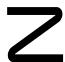
\includegraphics[keepaspectratio]{images/part003_35b408b4.jpg}}

注意：若 \((V,\pi)\) 是 A 的一个在 K 上非有限维的线性表示，则空间 \(\Theta_{\pi}(A)\) 未必包含在 \(\Theta(A)\) 中。

\subsection{半单代数的对偶}

设 \(\Theta^{\mathrm{ss}}(\mathrm{A})\) 是左 A-模 \(\Theta (\mathrm{A})\) 的底座，即（VIII, 第 65 页）\(\Theta (\mathrm{A})\) 的最大半单子模。我们用 \(\mathcal{S}_{\mathrm{K}}\) 表示在 K 上有限维的单（左）A-模的类所成的集。当 A 是 K 上一个有限次数的半单代数时，我们有 \(\mathrm{A}^{*} = \Theta (\mathrm{A}) = \Theta^{\mathrm{ss}}(\mathrm{A})\)，因为每个左 A-模都是半单的（VIII, 第 138 页，命题 4）。

定理 1. —— a) 集 \(\Theta^{\mathrm{ss}}(\mathrm{A})\) 由 A 的有限维半单表示的系数组成。它是 \(\mathrm{A}^*\) 的一个 (A,A)-子双模。

\begin{enumerate}
\def\labelenumi{\alph{enumi})}
\setcounter{enumi}{1}
\item
  对每个 \(S \in \mathcal{S}_{\mathrm{K}}\)，\(\Theta(A)\) 的 S 型同型分量等于 \(\Theta_{\mathrm{S}}(\mathrm{A})\)。左 A-模 \(\Theta^{\mathrm{ss}}(\mathrm{A})\) 是诸子模 \(\Theta_{\mathrm{S}}(\mathrm{A})\) 的直和，其中 S 取遍 \(\mathcal{S}_{\mathrm{K}}\)。
\item
  对 \(\mathcal{S}_{\mathrm{K}}\) 中每个 S，右 A-模 \(S^{*}\) 是单的，且 \(\Theta_{\mathrm{S}}(\mathrm{A})\) 是 \(S^{*}\) 型的同型分量（右 A-模 \(\Theta(\mathrm{A})\) 的）。把 S 映为 \(\operatorname{cl}(\mathrm{S}^{*})\) 的映射是从 \(\mathcal{S}_{\mathrm{K}}\) 到 K 上有限维单 \(A^{o}\) -模的类集的一个双射。
\item
  视为右 A-模时，\(\Theta (\mathrm{A})\) 的底座是 \(\Theta^{\mathrm{ss}}(\mathrm{A})\)。
\end{enumerate}

设 E 是一个在 K 上有限维的半单 A-模。E 的每个系数属于从 E 到 \(A^{*}\) 的某个 A-线性映射的像（VIII, 第 378 页，命题 2），因而属于 \(\Theta^{\mathrm{ss}}(\mathrm{A})\)。反之，设 \(f \in \Theta^{\mathrm{ss}}(\mathrm{A})\)。则 A-模 Af 在 K 上有限维且是半单的。由 VIII, 第 367 页的注，f 是 Af 的一个系数。

对 \(\mathcal{S}_{\mathrm{K}}\) 中每个 S，\(\Theta(\mathrm{A})\) 的 S 型同型分量由从 S 到 \(A^{*}\) 的 A-线性映射的像生成；因而由 VIII, 第 378 页，命题 2, a)，它等于 \(\Theta_{\mathrm{S}}(\mathrm{A})\)。另一方面，若 S 是一个在 K 上非有限维的单 A-模，则 \(\Theta(\mathrm{A})\) 的 S 型同型分量为零：事实上，\(\Theta(\mathrm{A})\) 的每个单子模都是单生成的，因此在 K 上有限维。由于 \(\Theta(\mathrm{A})\) 的底座是它的诸同型分量的直和（VIII, 第 65 页，命题 4），这就证明了 b)。

设 S 是一个在 K 上有限维的单 A-模。由于 K-向量空间 S 不约化为 0，\(S^{*}\) 亦然。设 E 是右 A-模 \(S^{*}\) 的一个子模；它在 S 中的正交 \(E'\) 是 S 的一个 A-子模。由于 S 是单的，我们或者有 \(E' = 0\)（此情形 \(E = S^{*}\)），或者有 \(E' = S\)（此情形 E = 0）。因此 \(S^{*}\) 是一个单右 A-模。

我们有 \(\Theta (\mathrm{A}^{\circ}) = \Theta (\mathrm{A})\)（VIII, 第 376 页）；我们把右 A-模等同于左 \(\mathrm{A}^{\circ}\) -模。由于 K 上每个有限维向量空间同构于它的双对偶，上述论证证明映射 \(\mathrm{S}\mapsto \mathrm{cl}(\mathrm{S}^{*})\) 是从 \(\mathcal{S}_{\mathrm{K}}\) 到 K 上有限维单 \(\mathrm{A}^{\circ}\) -模的类集的一个双射。现在，对 \(\mathcal{S}_{\mathrm{K}}\) 中的 S，\(\Theta (\mathrm{A}^{\circ})\) 的 \(\mathrm{S}^*\) 型同型分量等于 \(\Theta_{\mathrm{S}^*}(\mathrm{A}^{\circ})\)（由应用于代数 \(\mathrm{A}^{\circ}\) 的断言 b)），且我们有 \(\Theta_{\mathrm{S}^*}(\mathrm{A}^{\circ}) = \Theta_{\mathrm{S}}(\mathrm{A})\)。断言 c) 与 d) 随即得出。

推论 1. —— K 上每个有限维单 A-模都同构于 \(\Theta(A)\) 的一个 A-子模。

这由定理 1, b) 得出，因为对每个非零 A-模 E 我们有 \(\Theta_{\mathrm{E}}(\mathrm{A}) \neq 0\)。

推论 2. —— 若 K 上两个有限维单 A-模有一个公共的非零系数，则它们同构。

设 \(S_{1}\) 与 \(S_{2}\) 是 K 上有公共非零系数的有限维单 A-模。则我们有 \(\Theta_{S_{1}}(A) \cap \Theta_{S_{2}}(A) \neq 0\)。而 \(\Theta_{S_{1}}(A)\) 是 \(S_{1}\) 型的同型模，\(\Theta_{S_{2}}(A)\) 是 \(S_{2}\) 型的同型模。故 \(S_{1}\) 同构于 \(S_{2}\)。

由定理 1，\(\Theta^{\mathrm{ss}}(\mathrm{A})\) 是 \(\mathrm{A}^*\) 的一个 (A,A)-子双模，即诸 (A,A)-双模 \(\Theta_{\mathrm{S}}(\mathrm{A})\)（S 取遍 \(\mathcal{S}_{\mathrm{K}}\)）的直和。这些双模两两不同构，因为它们作为左 A-模已经不同构。

固定 \(\mathcal{S}_{\mathrm{K}}\) 中的一个 S。用 D 表示 \(\operatorname{End}_{\mathrm{A}}(\mathrm{S})\) 的反体，并把 S 视为一个右 D-模，\(S^{*}\) 视为一个左 D-模。在这些约定下，S 是一个 (A, D)-双模，\(S^{*}\) 是一个 (D, A)-双模，\(S \otimes_{D} S^{*}\) 是一个 (A, A)-双模。

命题 4. —— a) 存在一个群同态 \(\lambda_{\mathrm{S}}\)，它从 \(\mathrm{S} \otimes_{\mathrm{D}} \mathrm{S}^{*}\) 到 \(\Theta_{\mathrm{S}}(\mathrm{A})\)，由

\[
\lambda_ {\mathrm{S}} (x \otimes x ^ {*}) = c _ {\mathrm{S}} (x, x ^ {*})\tag{6}
\]

（对 \(x \in S\) 与 \(x^{*} \in S^{*}\)）刻画。这个映射是 (A, A)-双模的一个同构。

\begin{enumerate}
\def\labelenumi{\alph{enumi})}
\setcounter{enumi}{1}
\tightlist
\item
  (A, A)-双模 \(\Theta_{\mathrm{S}}(\mathrm{A})\) 是单的。
\end{enumerate}

映射 \(\gamma_{\mathrm{S}}: \mathrm{S} \otimes_{\mathrm{K}} \mathrm{S}^{*} \to \Theta_{\mathrm{S}}(\mathrm{A})\)（由公式 \(\gamma_{\mathrm{S}}(x \otimes x^{*}) = c_{\mathrm{S}}(x, x^{*})\) 刻画）是 (A, A)-线性的且是满射的，并满足 \(\gamma_{\mathrm{S}}(xd \otimes x^{*}) = \gamma_{\mathrm{S}}(x \otimes dx^{*})\)（对 \(x \in \mathrm{S}\)、\(x^{*} \in \mathrm{S}^{*}\) 与 \(d \in \mathrm{D}\)）。因此它定义了一个由公式 (6) 刻画的满射 (A, A)-线性映射 \(\lambda_{\mathrm{S}}: \mathrm{S} \otimes_{\mathrm{D}} \mathrm{S}^{*} \to \Theta_{\mathrm{S}}(\mathrm{A})\)。

我们来证明 \(S \otimes_{D} S^{*}\) 是一个单 (A, A)-双模。由 VIII, 第 63 页，推论 2，\(S \otimes_{D} S^{*}\) 的每个 (A, A)-子双模都具有形式 \(S \otimes_{D} H\)，其中 H 是 \(S^{*}\) 的一个 (D, A)-子双模。由于 \(S^{*}\) 是一个单右 A-模（VIII, 第 380 页，定理 1, c)），我们有 H = 0 或 \(H = S^{*}\)；断言得证。

同态 \(\lambda_{S}\) 是 (A, A)-线性的且非零；由于 \(S \otimes_{D} S^{*}\) 是一个单双模，\(\lambda_{S}\) 是单射的（VIII, 第 47 页，命题 2, a)）。

注. —— 当体 K 是代数闭的时，由 VIII, 第 47 页，定理 1，我们有 D = K，且 \(\lambda_{S}\) 是从 \(S \otimes_{K} S^{*}\) 到 \(\Theta_{\mathrm{S}}(\mathrm{A})\) 的 (A, A)-双模的一个同构。
